%%%%%%%%%%%%%%%%%%%%%%%%%%%%%%%%%%%%%%%%%%%%%%%%%%%%%%%%%%%%%%%%%%
%%%%%%%%%%%%%%%%%%%%%%%%%%%%%%%%%%%%%%%%%%%%%%%%%%%%%%%%%%%%%%%%%%
\chapter{Diagramme mit \texttt{ggplot2}}
\label{sec:ggplot}
%%%%%%%%%%%%%%%%%%%%%%%%%%%%%%%%%%%%%%%%%%%%%%%%%%%%%%%%%%%%%%%%%%
%%%%%%%%%%%%%%%%%%%%%%%%%%%%%%%%%%%%%%%%%%%%%%%%%%%%%%%%%%%%%%%%%%

\index{Grafik!ggplot2@\lstinline{ggplot2}}
\index[pack]{ggplot2@\lstinline{ggplot2}}
Mit dem Zusatzpaket \lstinline!ggplot2! lassen sich die in Kap.\ \ref{sec:graphics} vorgestellten Diagrammtypen ebenfalls erstellen. Dabei ist die Herangehensweise eine grundsätzlich andere: Während der Basisumfang von R für verschiedene Diagrammarten einzelne Funktionen bereitstellt, werden mit \lstinline!ggplot2! alle Diagrammtypen mit einem einheitlichen System erzeugt.\footnote{Dies orientiert sich an Ideen der \emph{grammar of graphics} \cite{Wilkinson2005} und basiert intern auf dem Paket \index[pack]{grid@\lstinline{grid}} \lstinline!grid! aus dem Basisumfang von R. Das Paket\index[pack]{lattice@\lstinline{lattice}} \lstinline!lattice! verfolgt vergleichbare Ziele wie \lstinline!ggplot2! und setzt ebenfalls auf \lstinline!grid! auf. Details erläutert \citeA{Murrell2005}.} Sind Diagramme des Basisumfangs analog zu einer Leinwand, auf der jede Funktion später nicht mehr änderbare Elemente aufmalt, repräsentiert \lstinline!ggplot2! alle Diagrammelemente explizit in einem Objekt. Erstellte Diagramme lassen sich über dieses Objekt weiter verändern, an Funktionen übergeben und speichern.

Zu den Vorteilen von \lstinline!ggplot2!-Diagrammen gegenüber jenen des Basisumfangs zählt, dass sie oft ästhetisch ansprechender sind und automatisch Legenden für alle verwendeten visuellen Attribute besitzen. Besser sind auch der einheitliche Zugang zu verschiedenen Diagrammtypen und die besonders einfache Möglichkeit, für alle Teilgruppen von Daten bedingte Diagramme in vielen Panels gleichzeitig darzustellen. Ein Nachteil ist die ungewohnte Syntax. Auch machen große Datenmengen die Darstellung langsam.

Eine detaillierte Einführung in \lstinline!ggplot2! findet sich bei \citeA{Wickham2009a} oder \citeA{Chang2013}. \citeA{Wilke2019} verwendet \lstinline!ggplot2! als Basis, um allgemein Grundlagen der Diagrammgestaltung zu erklären. Teils sind diese Bücher vollständig online erhältlich, teils zeigen sie auf einer Webseite zahlreiche Beispiele.\footnote{\url{https://ggplot2-book.org/} --
\url{https://r-graphics.org/} -- \url{https://serialmentor.com/dataviz/}\\Siehe auch das \lstinline!ggplot2! \emph{cheat sheet} unter \url{https://www.rstudio.com/resources/cheatsheets/}. Erweiterungen, etwa für neue Diagrammtypen, listet \url{http://www.ggplot2-exts.org/} auf. Das Paket \lstinline!gganimate!\index[pack]{gganimate@\lstinline{gganimate}} \cite{Pedersen2018} ermöglicht es Animationen zu erstellen.}

%%%%%%%%%%%%%%%%%%%%%%%%%%%%%%%%%%%%%%%%%%%%%%%%%%%%%%%%%%%%%%%%%%
%%%%%%%%%%%%%%%%%%%%%%%%%%%%%%%%%%%%%%%%%%%%%%%%%%%%%%%%%%%%%%%%%%
\section{Grundprinzip}
%%%%%%%%%%%%%%%%%%%%%%%%%%%%%%%%%%%%%%%%%%%%%%%%%%%%%%%%%%%%%%%%%%
%%%%%%%%%%%%%%%%%%%%%%%%%%%%%%%%%%%%%%%%%%%%%%%%%%%%%%%%%%%%%%%%%%

In \lstinline!ggplot2! wird ein Diagramm als Liste repräsentiert, die alle Informationen über die Darstellung beinhaltet und sich als Objekt speichern oder verändern lässt. \lstinline!ggplot!-Objekte erscheinen erst dann als Diagramm in einem device, wenn -- explizit oder implizit (Abschn.\ \ref{sec:printObject}) -- \lstinline!print(<<ggplot-Objekt>>)! aufgerufen wird.

%%%%%%%%%%%%%%%%%%%%%%%%%%%%%%%%%%%%%%%%%%%%%%%%%%%%%%%%%%%%%%%%%%
%%%%%%%%%%%%%%%%%%%%%%%%%%%%%%%%%%%%%%%%%%%%%%%%%%%%%%%%%%%%%%%%%%
\subsection{Grundschicht}
%%%%%%%%%%%%%%%%%%%%%%%%%%%%%%%%%%%%%%%%%%%%%%%%%%%%%%%%%%%%%%%%%%
%%%%%%%%%%%%%%%%%%%%%%%%%%%%%%%%%%%%%%%%%%%%%%%%%%%%%%%%%%%%%%%%%%

\index[func]{ggplot()@\lstinline{ggplot()}}
Für alle Diagrammtypen ist im ersten Schritte mit \lstinline!ggplot()! eine Grundschicht zu erzeugen, die die darzustellenden Daten festlegt und definiert, wie Eigenschaften der Daten in verschiedene visuelle Attribute umgesetzt werden. Einer Grundschicht lassen sich dann weitere Schichten hinzufügen, um ein konkretes Diagramm zu erhalten und Diagrammoptionen zu ändern.% Fügt man die Schichten schrittweise zu jeweils neuen Objekten zusammen, lässt sich für jeden Schritt kontrollieren, ob das Diagramm wie gewünscht aufgebaut wird.
\begin{lstlisting}
ggplot(<<Datensatz>>, aes(x=<<x-Koordinaten>>, y=<<y-Koordinaten>>,
                       colour=<<Variable>>,
                         fill=<<Variable>>,
                        shape=<<Faktor>>,
                     linetype=<<Faktor>>,
                        group=<<Faktor>>))
\end{lstlisting}

Als erstes Argument wird der Datensatz erwartet, aus dem die im Diagramm dargestellten Variablen stammen müssen. Bei Daten aus Messwiederholungen sollte der Datensatz im Long-Format vorliegen (Abschn.\ \ref{sec:reshape}). Das zweite Argument bestimmt mit der Funktion \lstinline!aes()!, welche Werte für die $x$- und $y$-Koordinaten herangezogen werden. Zusätzliche Argumente für \lstinline!aes()! kontrollieren die Zuordnung von weiteren Variablen zu visuellen Attributen der Diagrammelemente, die dann automatisch in der Legende erklärt werden.\footnote{\lstinline!vignette("ggplot2-specs")! erläutert die visuellen Attribute.} Zu beachten ist hierbei, dass alle Variablennamen ohne Anführungszeichen verwendet werden.\footnote{Wo dies notwendig ist, lässt sich alternativ \lstinline!aes_string()! mit Variablennamen in Anführungszeichen verwenden -- etwa wenn diese Elemente eines Vektors von Zeichenketten sind.}
\begin{itemize}
\item \lstinline!colour!: Eine übergebene Variable sorgt dafür, dass die Datenpunkte getrennt nach ihrer Ausprägung eingefärbt sind. Welche Farbe welcher Gruppe zugeordnet ist, wählt \lstinline!ggplot()! automatisch selbst (Abschn.\ \ref{sec:ggplotColour}). Möglich sind stetige Variablen wie auch Faktoren.
\item \lstinline!fill!: Bei flächigen Diagrammelementen -- etwa Säulen -- kontrolliert die übergebene Variable analog zu \lstinline!colour! deren Farbe.
\item \lstinline!shape!: Der übergebene Faktor bestimmt bei Punktdiagrammen die Art der Datenpunktsymbole (Abschn.\ \ref{sec:ggplotColour}).
\item \lstinline!linetype!: Der übergebene Faktor bestimmt den Linientyp bei Liniendiagrammen (Abschn.\ \ref{sec:ggplotColour}).
\item \lstinline!group!: Ein genannter Faktor sorgt dafür, dass in hinzugefügten Schichten jeweils alle Datenpunkte einer Gruppe (Faktorstufe) als zusammengehörig betrachtet werden. Unterschiedliche Gruppen werden dagegen getrennt behandelt, was etwa für Liniendiagramme oder boxplots relevant ist.\footnote{Übergibt man statt eines Faktors die \lstinline!1!, gehören alle Datenpunkte zusammen, z.\,B.\ für ein Liniendiagramm einer einzelnen Datenreihe.}
\end{itemize}

Die hier vorgestellten Beispiele verwenden die folgenden simulierten Daten.
\begin{lstlisting}
> Njk <- 50                          # Gruppengröße
> P   <- 3                           # Anzahl Stufen Gruppe
> Q   <- 2                           # Anzahl Stufen Geschlecht
> sex <- factor(rep(c("f", "m"), times=P*Njk))          # Geschlecht

# Gruppenzugehörigkeit
> group  <- factor(rep(c("control","placebo","treatment"), each=Q*Njk))
> sgComb <- interaction(sex, group)  # kombinierte Gruppenzugehörigkeit
> mood   <- round(rnorm(P*Q*Njk,     # Stimmung
+                       mean=c(85,80,110,90,130,100)[sgComb], sd=25))

> height <- rnorm(P*Q*Njk, mean=c(170, 180)[sex], sd=7) # Körpergröße
> rating <- factor(rbinom(Njk*P*Q, size=3,              # Zustimmung
+     prob=c(c(0.1,0.25,0.4,0.6,0.75,0.9))[sgComb]), levels=0:3,
+     labels=c("Not at all", "Somewhat", "Mostly", "Completely"))

# Gesamt-Datensatz
> myDf <- data.frame(sex, group, sgComb, mood, height, rating)
\end{lstlisting}

Als Grundschicht soll hier die Stimmung gegen die Körpergröße aufgetragen werden, wobei das Geschlecht die Farbe der Datenpunktsymbole und die Gruppenzugehörigkeit die Art der Datenpunktsymbole bestimmt. Die Grundschicht allein erzeugt ein leeres Diagramm.
\begin{lstlisting}
> library(ggplot2)                                      # für ggplot()
> ggplot(myDf, aes(x=height, y=mood, colour=sex, shape=group))
\end{lstlisting}

%%%%%%%%%%%%%%%%%%%%%%%%%%%%%%%%%%%%%%%%%%%%%%%%%%%%%%%%%%%%%%%%%%
%%%%%%%%%%%%%%%%%%%%%%%%%%%%%%%%%%%%%%%%%%%%%%%%%%%%%%%%%%%%%%%%%%
\subsection{Diagramme speichern}
%%%%%%%%%%%%%%%%%%%%%%%%%%%%%%%%%%%%%%%%%%%%%%%%%%%%%%%%%%%%%%%%%%
%%%%%%%%%%%%%%%%%%%%%%%%%%%%%%%%%%%%%%%%%%%%%%%%%%%%%%%%%%%%%%%%%%

Mit den in Abschn.\ \ref{sec:saveDiag} vorgestellten Funktionen wie \index[func]{pdf()@\lstinline{pdf()}} \lstinline!pdf()! oder \index[func]{jpeg()@\lstinline{jpeg()}} \lstinline!jpeg()! lassen sich ebenfalls \lstinline!ggplot!-Objekte speichern. Eine bequeme Alternative dazu ist \index[func]{ggsave()@\lstinline{ggsave()}} \lstinline!ggsave()!.
\begin{lstlisting}
ggsave("<<Dateiname>>", plot, device, width=<<Breite>>, height=<<Höhe>>,
       units="<<Maßeinheit>>", dpi=<<Auflösung>>)
\end{lstlisting}

Nach dem Dateinamen im ersten Argument kann optional ein \lstinline!ggplot!-Objekt als zweites Argument \lstinline!plot! übergeben werden. Fehlt dies, speichert die Funktion automatisch das letzte dargestellte \lstinline!ggplot!-Diagramm. Anhand der gewählten Endung des Dateinamens (etwa \lstinline!"<<Name>>.pdf"!) wählt \lstinline!ggsave()! selbst automatisch das passende Grafikformat. Dies kann aber auch für \lstinline!device! explizit angegeben werden. Breite und Höhe der Grafikdatei lassen sich über \lstinline!width! und \lstinline!height! kontrollieren, wobei die gemeinte Maßeinheit für \lstinline!units! zu nennen ist -- Voreinstellung ist \lstinline!"in"! für inch, andere Möglichkeiten sind \lstinline!"cm"! und \lstinline!"mm"!. Die Auflösung beträgt in der Voreinstellung 300 dpi (\emph{dots per inch}) und kann über \lstinline!dpi! erhöht oder gesenkt werden.

%%%%%%%%%%%%%%%%%%%%%%%%%%%%%%%%%%%%%%%%%%%%%%%%%%%%%%%%%%%%%%%%%%
%%%%%%%%%%%%%%%%%%%%%%%%%%%%%%%%%%%%%%%%%%%%%%%%%%%%%%%%%%%%%%%%%%
\section{Diagrammtypen}
%%%%%%%%%%%%%%%%%%%%%%%%%%%%%%%%%%%%%%%%%%%%%%%%%%%%%%%%%%%%%%%%%%
%%%%%%%%%%%%%%%%%%%%%%%%%%%%%%%%%%%%%%%%%%%%%%%%%%%%%%%%%%%%%%%%%%

Jede der folgenden Funktionen fügt einer mit \lstinline!ggplot()! erstellten Grundschicht einen konkreten Diagrammtyp hinzu (für weitere vgl.\ \citeNP{Wickham2009a}), wenn sie mit dieser Schicht über \lstinline!+! verknüpft wird.\footnote{Die ungewöhnliche Syntax ist möglich, weil der Operator \lstinline!+! eine Funktion ist, \lstinline!a + b! also in \lstinline!\"+\"(a, b)! übersetzt wird (Abschn.\ \ref{sec:funcParam}). Weiter ist \lstinline!\"+\"()! generisch, kann sich also für \lstinline!ggplot!-Objekte anders als für Zahlen verhalten (Abschn.\ \ref{sec:funcGeneric}).} Dafür besitzen die genannten Funktionen eigene Argumente, um Eigenschaften zu kontrollieren, die spezifisch für den jeweiligen Diagrammtyp sind (s.\,u.\ für Beispiele und die jeweils zugehörige Hilfe-Seite für Details).

\begin{itemize}
\item \index[func]{geom_point()@\lstinline{geom_point()}} \lstinline!geom_point()! für ein Punkt- oder Streudiagramm
\item \index[func]{geom_bar()@\lstinline{geom_bar()}} \lstinline!geom_bar()! für ein Säulendiagramm
%\item \index[func]{geom_dotplot()@\lstinline{geom_dotplot()}} \lstinline!geom_dotplot()! für 
\item \index[func]{geom_histogram()@\lstinline{geom_histogram()}} \lstinline!geom_histogram()! für ein Histogramm
\item \index[func]{geom_density()@\lstinline{geom_density()}} \lstinline!geom_density()! für einen Kerndichteschätzer
\item \index[func]{geom_line()@\lstinline{geom_line()}} \lstinline!geom_line()! für ein Liniendiagramm
\item \index[func]{geom_boxplot()@\lstinline{geom_boxplot()}} \lstinline!geom_boxplot()! für einen boxplot
\end{itemize}

Die Diagrammtypen lassen sich auch kombinieren: So kann etwa einer Grundschicht sowohl ein boxplot als auch ein Punktdiagramm für die Rohdaten hinzugefügt werden, die das Diagramm dann beide darstellt.

Alle \lstinline!geom_<<Name>>()! Funktionen verwenden in der Voreinstellung den in der Grundschicht definierten Datensatz. Sie können aber auch auf einen eigenen Datensatz Bezug nehmen, der für das Argument \lstinline!data! zu nennen ist. Analog lässt sich über \lstinline!aes()! eine eigene Zuordnung von Variablen des Datensatzes zu visuellen Attributen des Diagramms festlegen.

%%%%%%%%%%%%%%%%%%%%%%%%%%%%%%%%%%%%%%%%%%%%%%%%%%%%%%%%%%%%%%%%%%
%%%%%%%%%%%%%%%%%%%%%%%%%%%%%%%%%%%%%%%%%%%%%%%%%%%%%%%%%%%%%%%%%%
\subsection{Punkt-, Streu- und Liniendiagramme}
\label{sec:ggplotPoint}
%%%%%%%%%%%%%%%%%%%%%%%%%%%%%%%%%%%%%%%%%%%%%%%%%%%%%%%%%%%%%%%%%%
%%%%%%%%%%%%%%%%%%%%%%%%%%%%%%%%%%%%%%%%%%%%%%%%%%%%%%%%%%%%%%%%%%

Als Beispiel soll zunächst mit\index[func]{geom_point()@\lstinline{geom_point()}} \lstinline!geom_point()! ein Streudiagramm erzeugt werden (Abb.\ \ref{fig:ggplot01}).
\begin{lstlisting}
# füge Grundschicht Streudiagramm mit größeren Datenpunktsymbolen hinzu
> ggplot(myDf, aes(x=height, y=mood, colour=sex, shape=group)) +
+     geom_point(size=3)
\end{lstlisting}

Das mit \lstinline!geom_line()! erzeugte Liniendiagramm zeigt die Gruppenmittelwerte der Stimmung getrennt für Männer und Frauen (Abb.\ \ref{fig:ggplot01}). Dafür soll zunächst mit \lstinline!aggregate()! (Abschn.\ \ref{sec:aggregate}) ein geeigneter Datensatz erzeugt werden.
\begin{lstlisting}
> (groupM <- aggregate(mood ~ sex + group, data=myDf, FUN=mean))
  sex     group      mood
1   f   control  76.06667
2   m   control  82.60000
3   f   placebo 118.76667
4   m   placebo  95.60000
5   f treatment 132.70000
6   m treatment 103.93333

> ggplot(groupM,
+        aes(x=group, y=mood, color=sex, shape=sex, group=sex)) +
+     geom_point() +
+     geom_line()
\end{lstlisting}

\begin{figure}[ht]
\centering
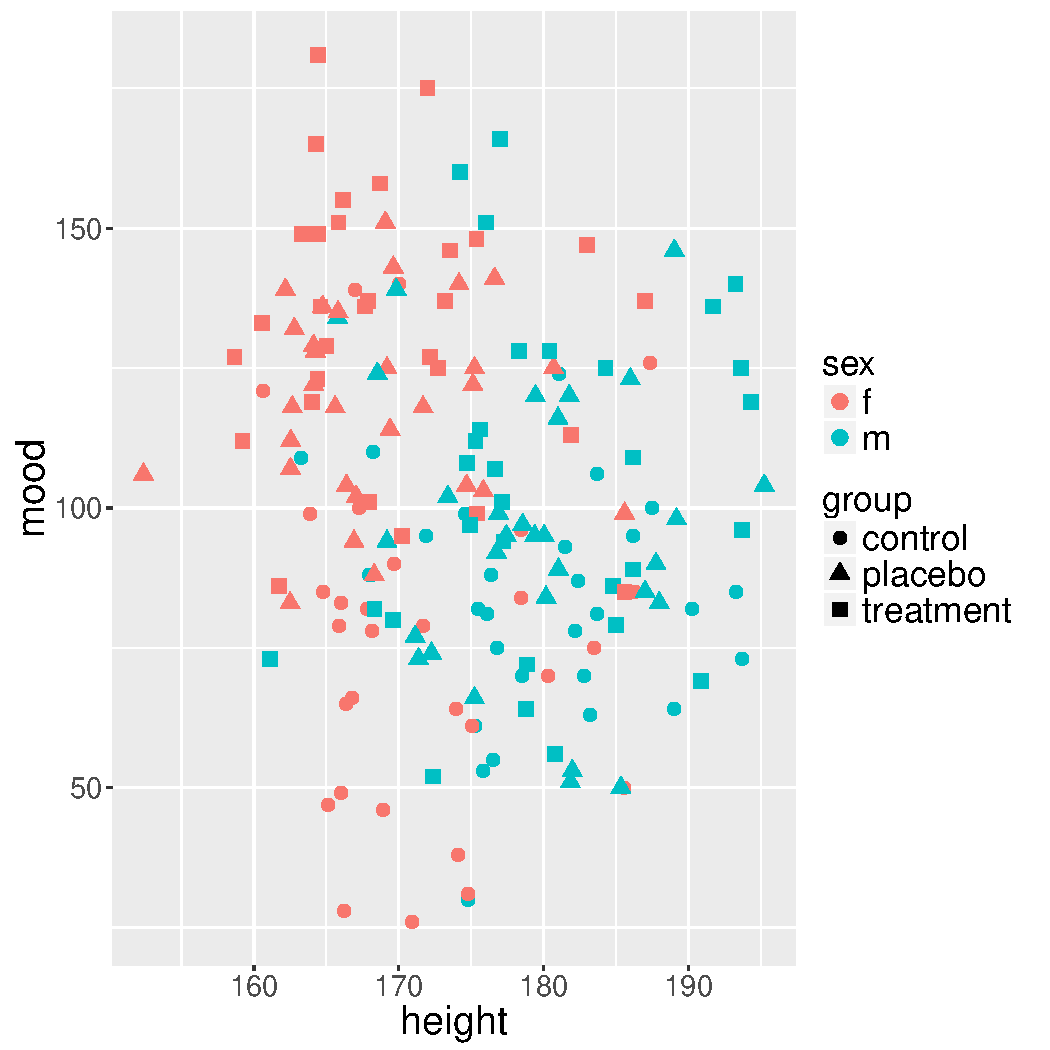
\includegraphics[width=6.25cm]{ggplot01a}
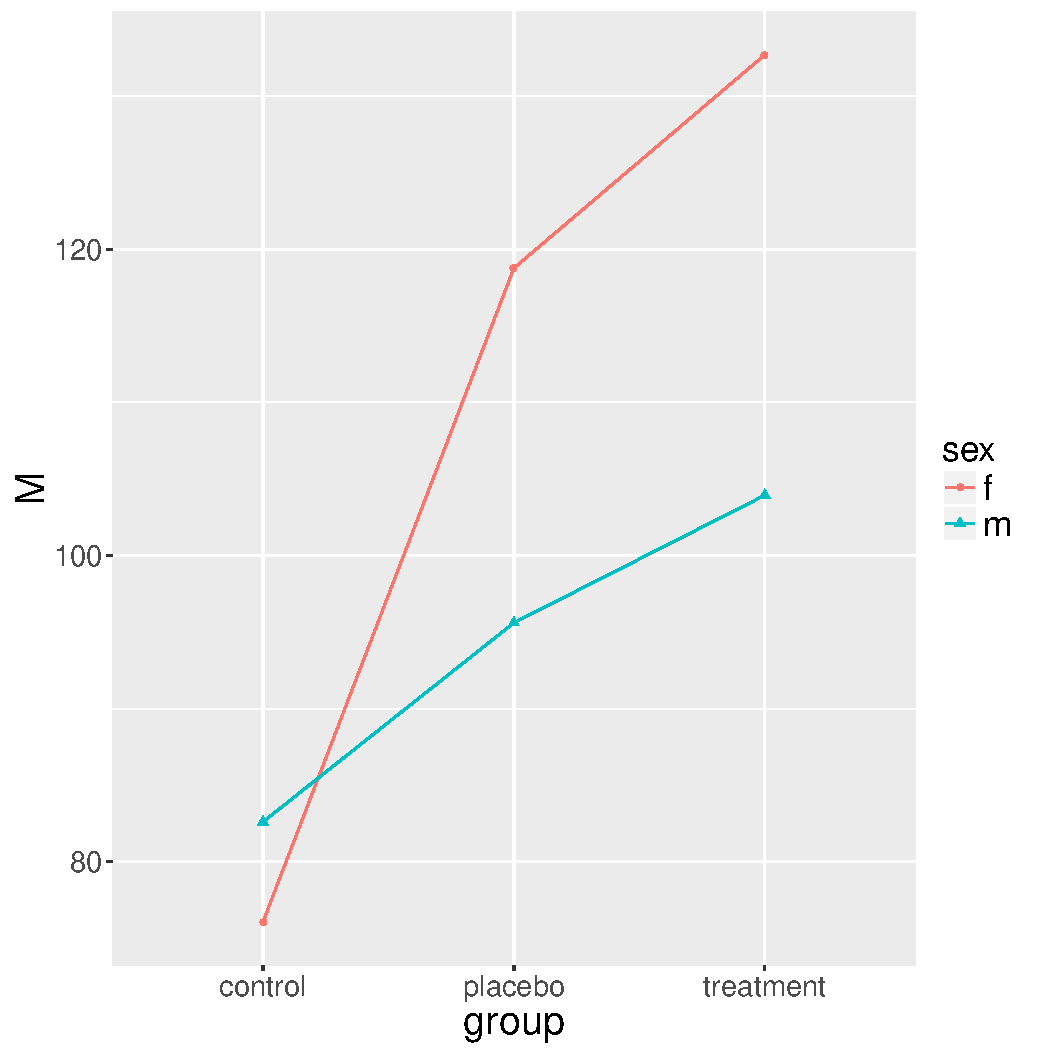
\includegraphics[width=6.25cm]{ggplot01b}
\vspace*{-0.5em}
\caption{Streudiagramm mit \lstinline!geom_point()! und Liniendiagramm mit \lstinline!geom_line()!}
\label{fig:ggplot01}
\end{figure}

%%%%%%%%%%%%%%%%%%%%%%%%%%%%%%%%%%%%%%%%%%%%%%%%%%%%%%%%%%%%%%%%%%
%%%%%%%%%%%%%%%%%%%%%%%%%%%%%%%%%%%%%%%%%%%%%%%%%%%%%%%%%%%%%%%%%%
\subsection{Säulendiagramm}
%%%%%%%%%%%%%%%%%%%%%%%%%%%%%%%%%%%%%%%%%%%%%%%%%%%%%%%%%%%%%%%%%%
%%%%%%%%%%%%%%%%%%%%%%%%%%%%%%%%%%%%%%%%%%%%%%%%%%%%%%%%%%%%%%%%%%

Für ein Säulendiagramm mit\index[func]{geom_bar()@\lstinline{geom_bar()}} \lstinline!geom_bar()! ist im vorherigen Aufruf von \lstinline!ggplot(..., aes(x=<<Variable>>))! für \lstinline!x! die Variable anzugeben, die die Höhe der Säulen bestimmt. In der üblichen Verwendung ist dies eine kategoriale Variable, deren absolute Häufigkeiten von \lstinline!geom_bar(stat="count")! automatisch ausgezählt und als Säulenhöhe visualisiert werden. Relative Häufigkeiten erhält man mit \lstinline!geom_bar(stat="count", aes(y=(..count..) / sum(..count..)))!.\footnote{\label{ftn:ggplotCount}\lstinline!..count..! ist der Name einer mit \lstinline!stat="count"! intern erzeugten Variable mit den berechneten Gruppenhäufigkeiten, auf die man innerhalb des Aufrufs von \lstinline!aes()! Zugriff hat.}

Dagegen stellt \lstinline!geom_bar(stat="identity")! die nicht weiter aggregierten Werte von \lstinline!x! selbst als Säulenhöhe dar -- etwa wenn dies bereits vorher berechnete Häufigkeiten sind (Abb.\ \ref{fig:ggplot02}). \lstinline!geom_bar(position=position_dodge())! sorgt für ein gruppiertes Säulendiagramm, während die Voreinstellung mit \lstinline!position_stack()! ein gestapeltes ist (Abschn.\ \ref{sec:ggplotPos}). Sollen im gestapelten Säulendiagramm alle Säulen auf die Länge 1 normiert sein, damit die Segmente die bedingten relativen Anteile der ausgezählten kategorialen Variable darstellen, ist \lstinline!position_fill()! zu verwenden (Abb.\ \ref{fig:ggplot07}). Abschnitt \ref{sec:ggplotAxis} zeigt, wie Achsenbeschriftungen angepasst werden können.
\begin{lstlisting}
# gestapeltes Säulendiagramm
> ggplot(myDf, aes(x=rating, group=sex, fill=sex)) +
+     geom_bar(stat="count", position=position_stack())

# gestapeltes und normiertes Säulendiagramm
> ggplot(myDf, aes(x=rating, group=sex, fill=sex)) +
+     geom_bar(stat="count",
+              aes(y=(..count..) / sum(..count..)),
+              position=position_fill())

# gruppiertes Säulendiagramm
> ggplot(myDf, aes(x=rating, group=sex, fill=sex)) +
+     geom_bar(stat="count",
+              aes(y=(..count..) / sum(..count..)),
+              position=position_dodge())
\end{lstlisting}

\begin{figure}[ht]
\centering
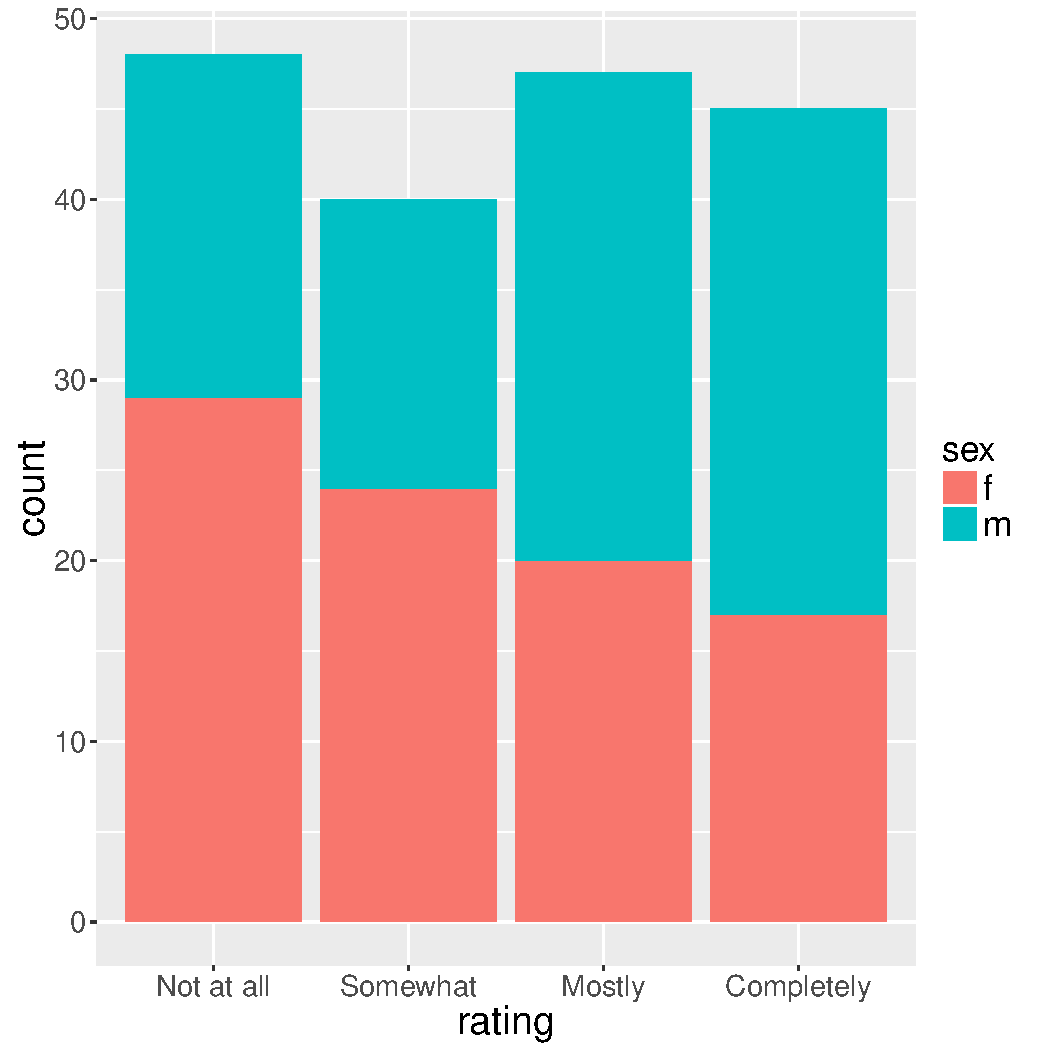
\includegraphics[width=6.25cm]{ggplot02a}
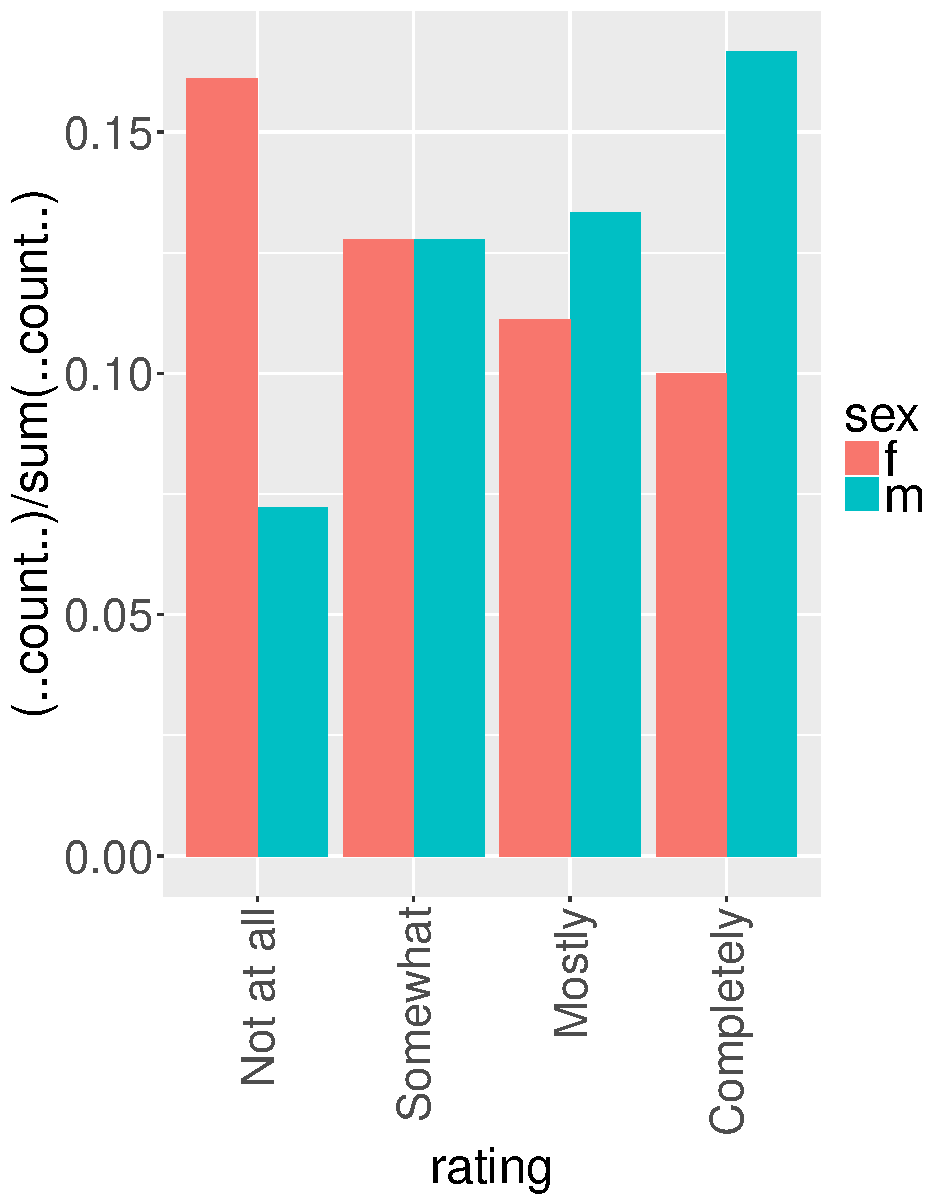
\includegraphics[width=6.25cm]{ggplot02b}
\vspace*{-0.5em}
\caption{Gestapeltes Säulendiagramm der absoluten Häufigkeiten sowie gruppiertes Säulendiagramm der relativen Häufigkeiten mit \lstinline!geom_bar()!. Für senkrecht orientierte Beschriftungen der $x$-Achse s.\ Abschn.\ \ref{sec:ggplotAxis}.}
\label{fig:ggplot02}
\end{figure}

%%%%%%%%%%%%%%%%%%%%%%%%%%%%%%%%%%%%%%%%%%%%%%%%%%%%%%%%%%%%%%%%%%
%%%%%%%%%%%%%%%%%%%%%%%%%%%%%%%%%%%%%%%%%%%%%%%%%%%%%%%%%%%%%%%%%%
\subsection{Histogramm}
%%%%%%%%%%%%%%%%%%%%%%%%%%%%%%%%%%%%%%%%%%%%%%%%%%%%%%%%%%%%%%%%%%
%%%%%%%%%%%%%%%%%%%%%%%%%%%%%%%%%%%%%%%%%%%%%%%%%%%%%%%%%%%%%%%%%%

Bei einem Histogramm mit\index[func]{geom_histogram()@\lstinline{geom_histogram()}} \lstinline!geom_histogram()! ist im vorherigen Aufruf \lstinline!ggplot(..., aes(x=<<Variable>>))! für \lstinline!x! die Variable anzugeben, deren Häufigkeit von Werte-Intervallen das Histogramm darstellt. Um die geschätzte Dichte (die relative Häufigkeit geteilt durch die Intervallbreite) statt der absoluten Häufigkeiten der Kategorien darzustellen, kann man \lstinline!geom_histogram(aes(y=..density..))! verwenden.\footnote{Analog zu Fußnote \ref{ftn:ggplotCount} ist \lstinline!..density..! der Name einer intern berechneten Variable, auf die man innerhalb von \lstinline!aes()! Zugriff hat.} In \lstinline!geom_histogram()! lässt sich über \lstinline!binwidth=<<Breite>>! die Breite der Intervalle kontrollieren, alternativ über \lstinline!bins=<<Anzahl>>! ihre Anzahl (Abb.\ \ref{fig:ggplot03}).
\begin{lstlisting}
> ggplot(myDf, aes(x=mood)) +
+     geom_histogram(bins=30))
\end{lstlisting}

Weil die Form eines Histogramms abhängig ist von der willkürlichen Wahl der Intervallanzahl und der Intervallgrenzen, ist ein zusätzlich dargestellter Kerndichteschätzer oft sinnvoll. Dieser lässt sich mit \lstinline!geom_density()!\index[func]{geom_density()@\lstinline{geom_density()}} hinzufügen (Abb.\ \ref{fig:ggplot03}). Die Farbwahl erläutert Abschn.\ \ref{sec:ggplotColour}.
\begin{lstlisting}
> ggplot(myDf, aes(x=mood)) +
+     geom_histogram(aes(y=..density..)) +
+     geom_density(color="darkgrey", fill="grey", alpha=0.6))
\end{lstlisting}

\begin{figure}[ht]
\centering
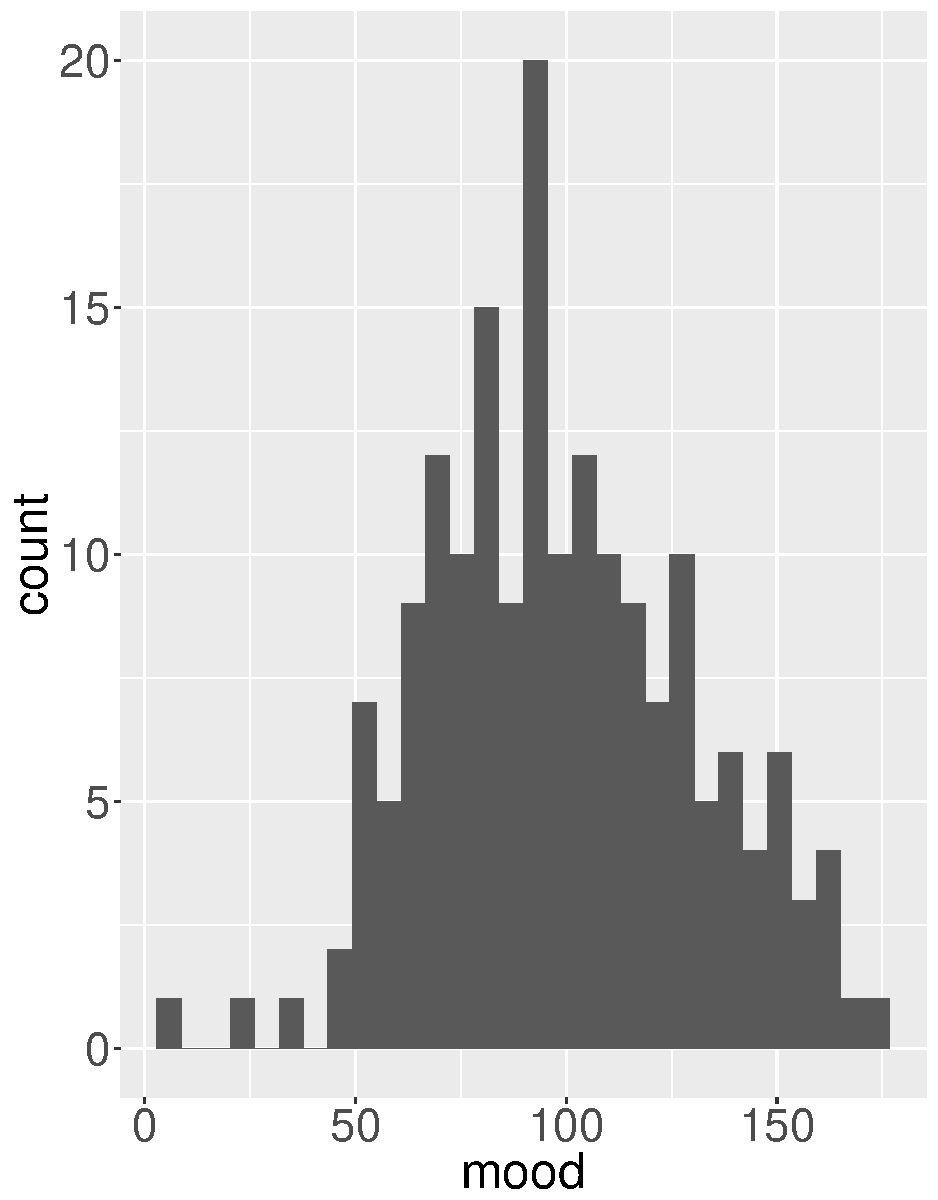
\includegraphics[width=6.25cm]{ggplot03a}
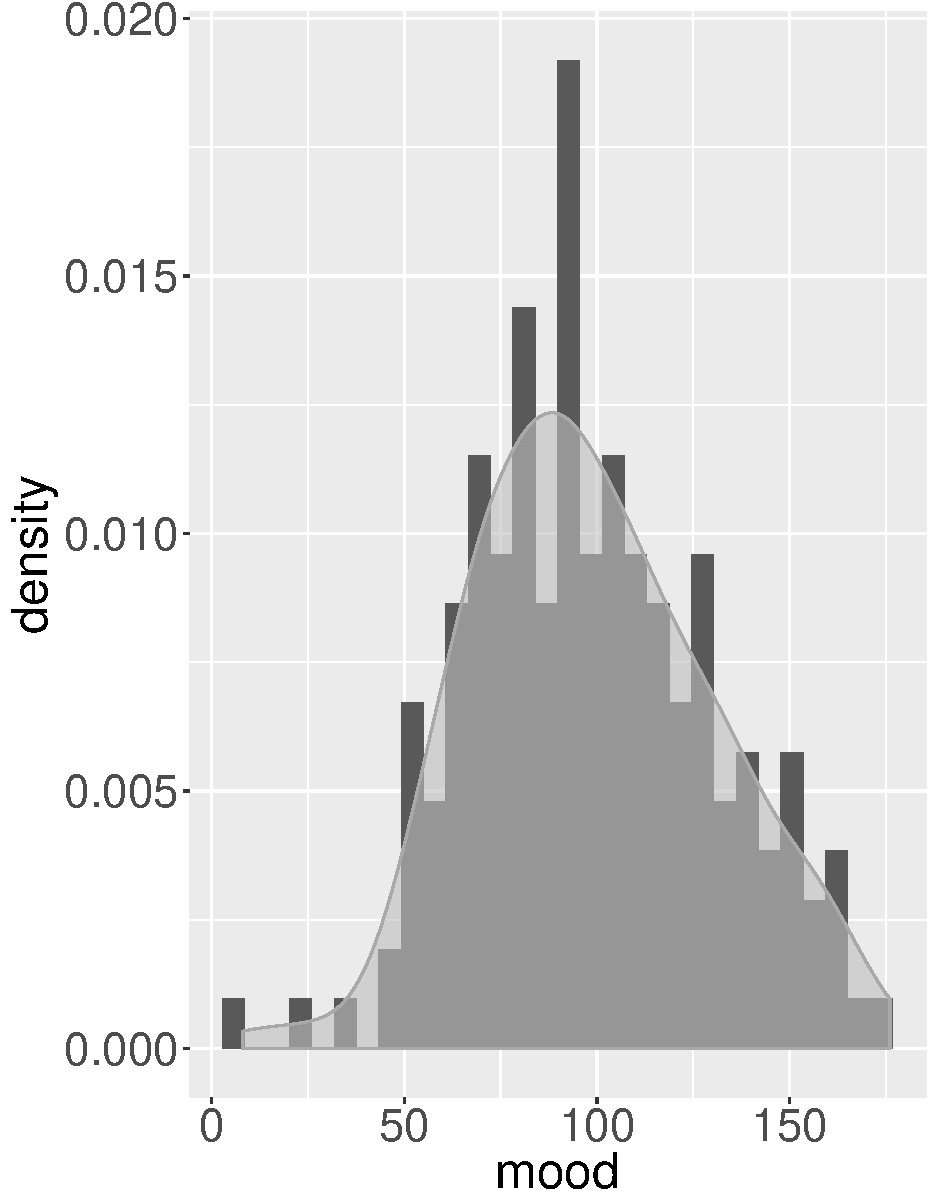
\includegraphics[width=6.25cm]{ggplot03b}
\vspace*{-0.5em}
\caption{Histogramm der absoluten Häufigkeiten mit \lstinline!geom_histogram()! sowie Dichte-Histogramm und Kerndichteschätzer mit \lstinline!geom_density()!}
\label{fig:ggplot03}
\end{figure}

%%%%%%%%%%%%%%%%%%%%%%%%%%%%%%%%%%%%%%%%%%%%%%%%%%%%%%%%%%%%%%%%%%
%%%%%%%%%%%%%%%%%%%%%%%%%%%%%%%%%%%%%%%%%%%%%%%%%%%%%%%%%%%%%%%%%%
\subsection{Boxplot}
\label{sec:ggplotBoxplot}
%%%%%%%%%%%%%%%%%%%%%%%%%%%%%%%%%%%%%%%%%%%%%%%%%%%%%%%%%%%%%%%%%%
%%%%%%%%%%%%%%%%%%%%%%%%%%%%%%%%%%%%%%%%%%%%%%%%%%%%%%%%%%%%%%%%%%

\lstinline!geom_boxplot()!\index[func]{geom_boxplot()@\lstinline{geom_boxplot()}} erzeugt einen boxplot (Abschn.\ \ref{sec:boxplot}), wobei im vorherigen Aufruf von \lstinline!ggplot()! innerhalb von \lstinline!aes(x=<<Faktor>>, y=<<Variable>>, ...))! für \lstinline!x! ein Faktor zu übergeben ist, für dessen Stufen separate boxplots angezeigt werden. Diese boxplots stellen die Kennwerte der für \lstinline!y! genannten Variable in den Gruppen dar (Abb.\ \ref{fig:ggplot04}). Abschnitt \ref{sec:ggplotLegend} zeigt, wie die hier unnötige Legende entfernt werden kann.
\begin{lstlisting}
> ggplot(myDf, aes(x=sex, y=height, fill=sex)) +
+     geom_boxplot()
\end{lstlisting}

Da boxplots wichtige Eigenschaften der Verteilung wie etwa Multimodalität nicht repräsentieren können, ist es oft sinnvoll, zusätzlich die Rohdaten darzustellen. \lstinline!geom_beeswarm()!\index[func]{geom_beeswarm()@\lstinline{geom_beeswarm()}} aus dem Paket \lstinline!ggbeeswarm!\index[pack]{ggbeeswarm@\lstinline{ggbeeswarm}} \cite{Clarke2017} zeigt alle einzelnen Datenpunkte, wobei die horizontale Position so versetzt gewählt wird, dass die Verteilungsform gut ersichtlich ist (Abb.\ \ref{fig:ggplot04}). Damit Ausreißer nicht doppelt dargestellt werden, sollte man sie im Aufruf von \lstinline!geom_boxplot()! mit der Option \lstinline!outlier.shape=NULL! ausblenden.
\begin{lstlisting}
> library(ggbeeswarm)                    # für geom_beeswarm()
> ggplot(myDf, aes(x=sex, y=height, fill=sex)) +
+     geom_boxplot(outlier.shape=NULL) + # boxplot: outlier ausblenden
+     geom_beeswarm(alpha=0.5)           # mit simulierter Transparenz
\end{lstlisting}

\begin{figure}[ht]
\centering
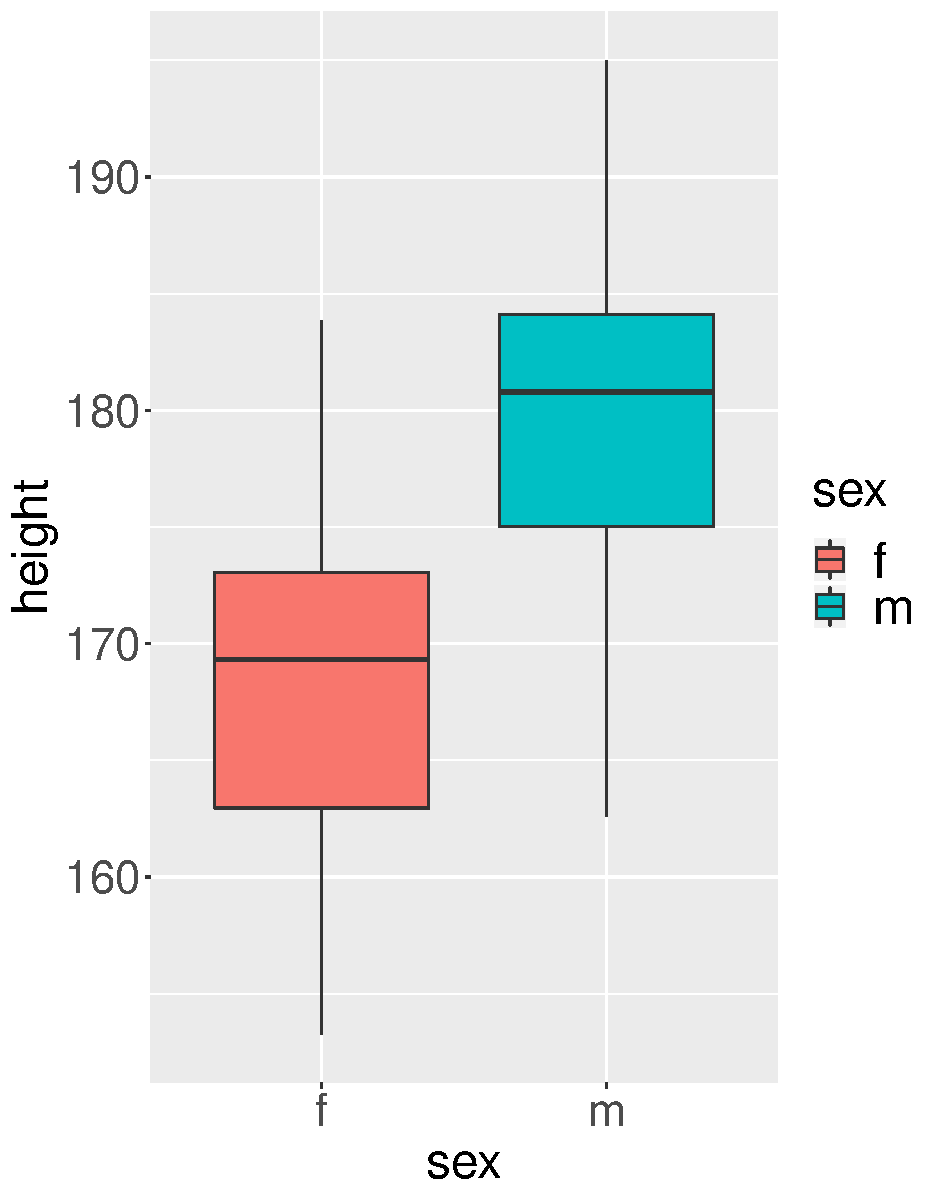
\includegraphics[width=6.25cm]{ggplot04a}
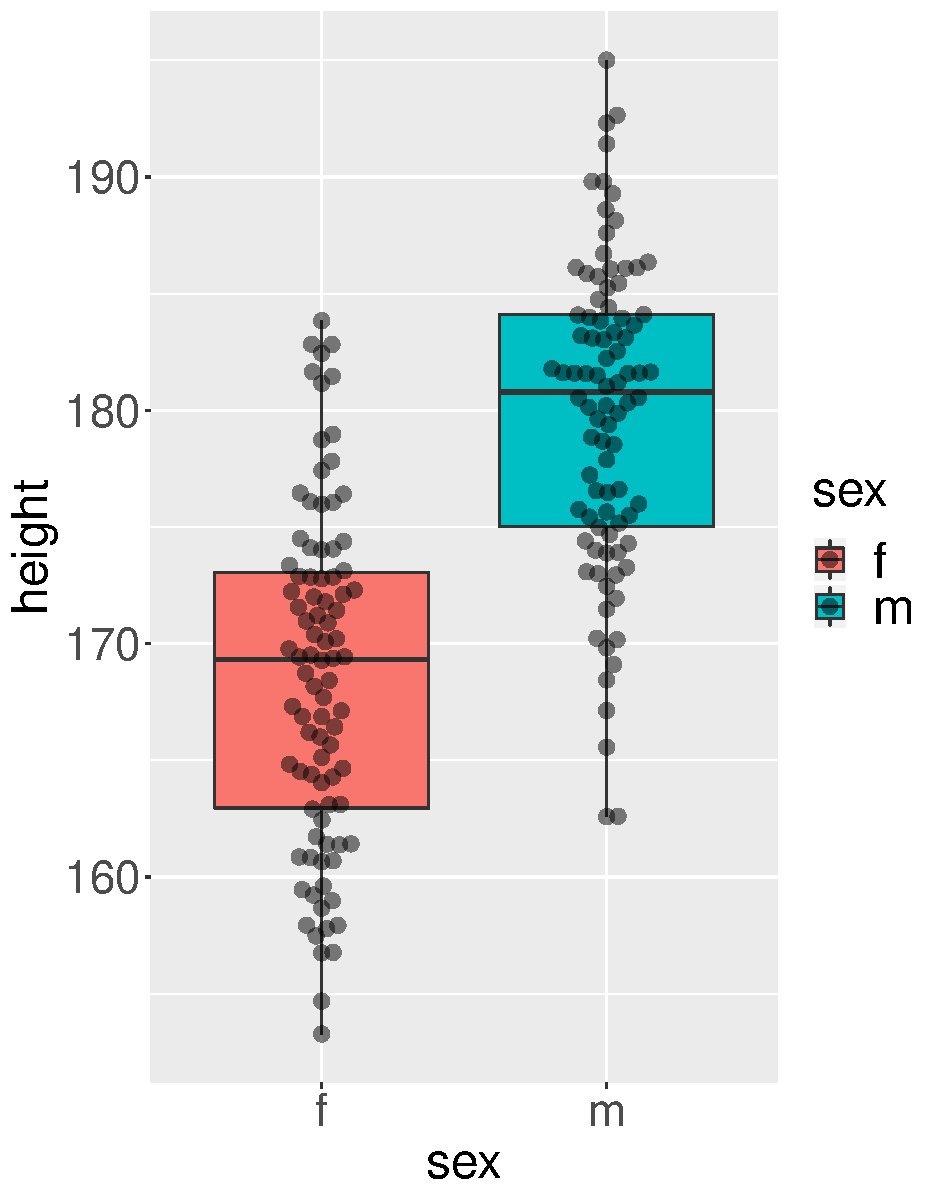
\includegraphics[width=6.25cm]{ggplot04b}
\vspace*{-0.5em}
\caption{Nach Geschlecht getrennte boxplots mit \lstinline!geom_boxplot()! sowie Rohdaten mit \lstinline!geom_beeswarm()!}
\label{fig:ggplot04}
\end{figure}

%%%%%%%%%%%%%%%%%%%%%%%%%%%%%%%%%%%%%%%%%%%%%%%%%%%%%%%%%%%%%%%%%%
%%%%%%%%%%%%%%%%%%%%%%%%%%%%%%%%%%%%%%%%%%%%%%%%%%%%%%%%%%%%%%%%%%
\subsection{Quantil-Quantil-Diagramm}
\label{sec:ggplotQQ}
%%%%%%%%%%%%%%%%%%%%%%%%%%%%%%%%%%%%%%%%%%%%%%%%%%%%%%%%%%%%%%%%%%
%%%%%%%%%%%%%%%%%%%%%%%%%%%%%%%%%%%%%%%%%%%%%%%%%%%%%%%%%%%%%%%%%%

Quantil-Quantil-Diagramme vergleichen eine empirische mit einer theoretisch vermuteten Verteilung mit Hilfe der jeweiligen Quantile zu denselben Wahrscheinlichkeiten, oder vergleichen analog zwei empirische Verteilungen (Abschn.\ \ref{sec:qq}). Die Diagramme werden durch \lstinline!geom_qq()!\index[func]{geom_qq()@\lstinline{geom_qq()}} erzeugt, woraufhin \lstinline!geom_qq_line()!\index[func]{geom_qq_line()@\lstinline{geom_qq_line()}} eine entsprechende Referenzlinie hinzufügt (Abb.\ \ref{fig:ggplot031}). Im vorausgehenden Aufruf von \lstinline!ggplot()! muss dafür innerhalb von \lstinline!aes()! die Option \lstinline!sample! die Variable definieren, deren empirische Quantile gegen die theoretischen Qantile -- in der Voreinstellung die der Standardnormalverteilung -- in einem Streudiagramm aufgetragen werden.
\begin{lstlisting}
> ggplot(myDf, aes(sample=height)) +
+     geom_qq() +
+     geom_qq_line(color="blue")
\end{lstlisting}

Für den Vergleich mit einer anderen theoretischen Verteilung kann deren Quantilfunktion in \lstinline!geom_qq()! und \lstinline!geom_qq_line()! an das Argument \lstinline!distribution! übergeben werden. Zusätzliche Parameter für diese Funktion sind in Form einer Liste mit entsprechend benannten Komponenten für das Argument \lstinline!dparams! zu nennen.\footnote{Für die Schätzung der Parameter geläufiger Verteilungen s.\ Abschn.\ \ref{sec:fitDistr}.}
\begin{lstlisting}
> parL <- list(df=10, ncp=0)               # Parameter für t-Verteilung
> ggplot(myDf, aes(sample=height)) +
+     geom_qq(distribution=qt, dparams=parL) +
+     geom_qq_line(color="blue", distribution=qt, dparams=parL)
\end{lstlisting}

Für den Vergleich der Quantile zweier empirischer Verteilungen sind zunächst mit \lstinline!ppoints()! die zu einem Quantil gehörende Werte der empirischen kumulierten Häufigkeitsverteilung als Schätzung der Verteilungsfunktion zu bilden. Als Argument kann die gewünschte Anzahl von Werten oder ein Vektor übergeben werden, dessen Länge dann die Anzahl bestimmt. Nach Berechnung der zugehörigen Quantile in beiden relevanten Variablen für die von \lstinline!ppoints()! ausgegebenen Werte kann das Streudiagramm der Quantile manuell erstellt werden.
\begin{lstlisting}
> probs <- ppoints(50)
> qDat  <- data.frame(qmood=quantile(myDf$mood, probs),
+                     qheight=quantile(myDf$height, probs))

> ggplot(qDat, aes(x=qmood, y=qheight)) +
+     geom_point() +
+     xlab("Quantiles mood") +
+     ylab("Quantiles height")
\end{lstlisting}

\begin{figure}[ht]
\centering
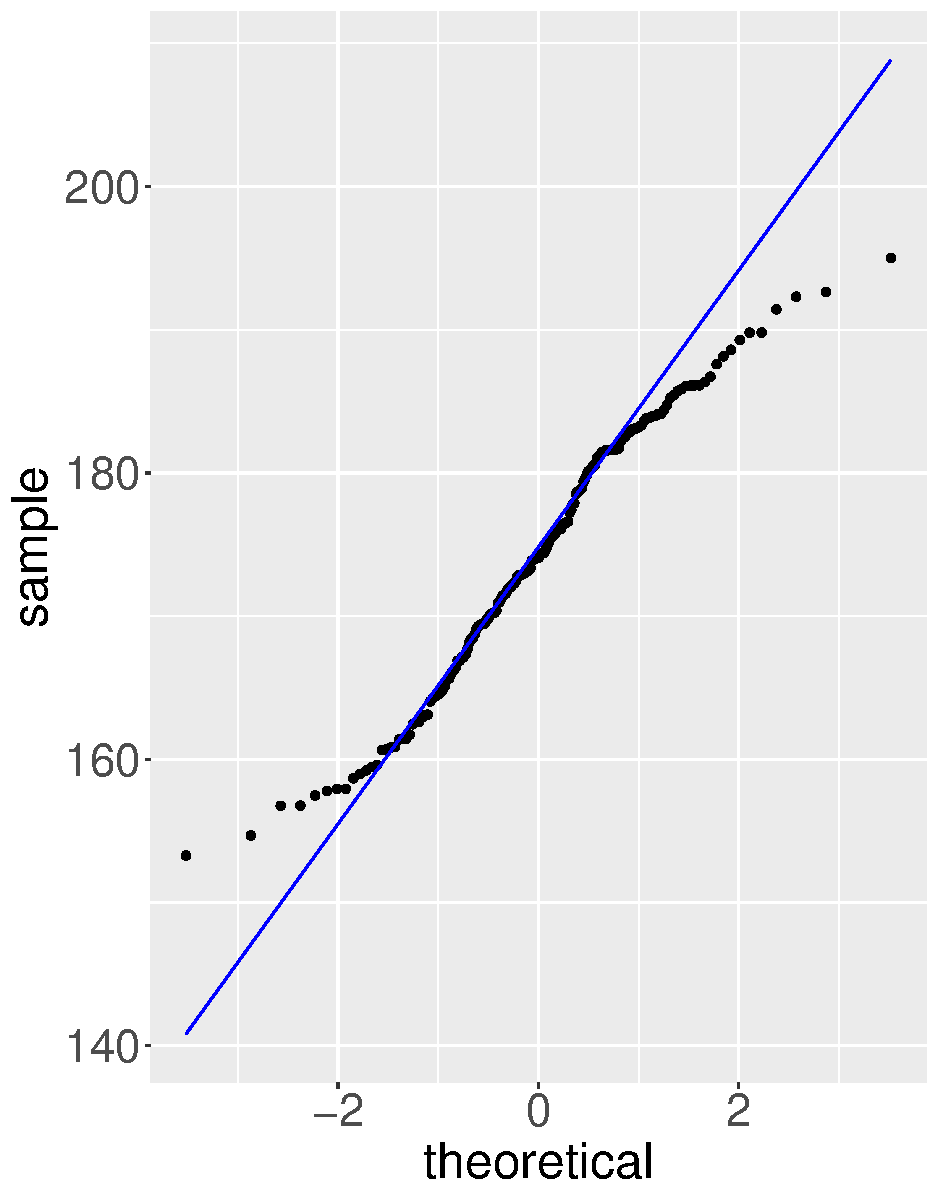
\includegraphics[width=6.25cm]{ggplot031a}
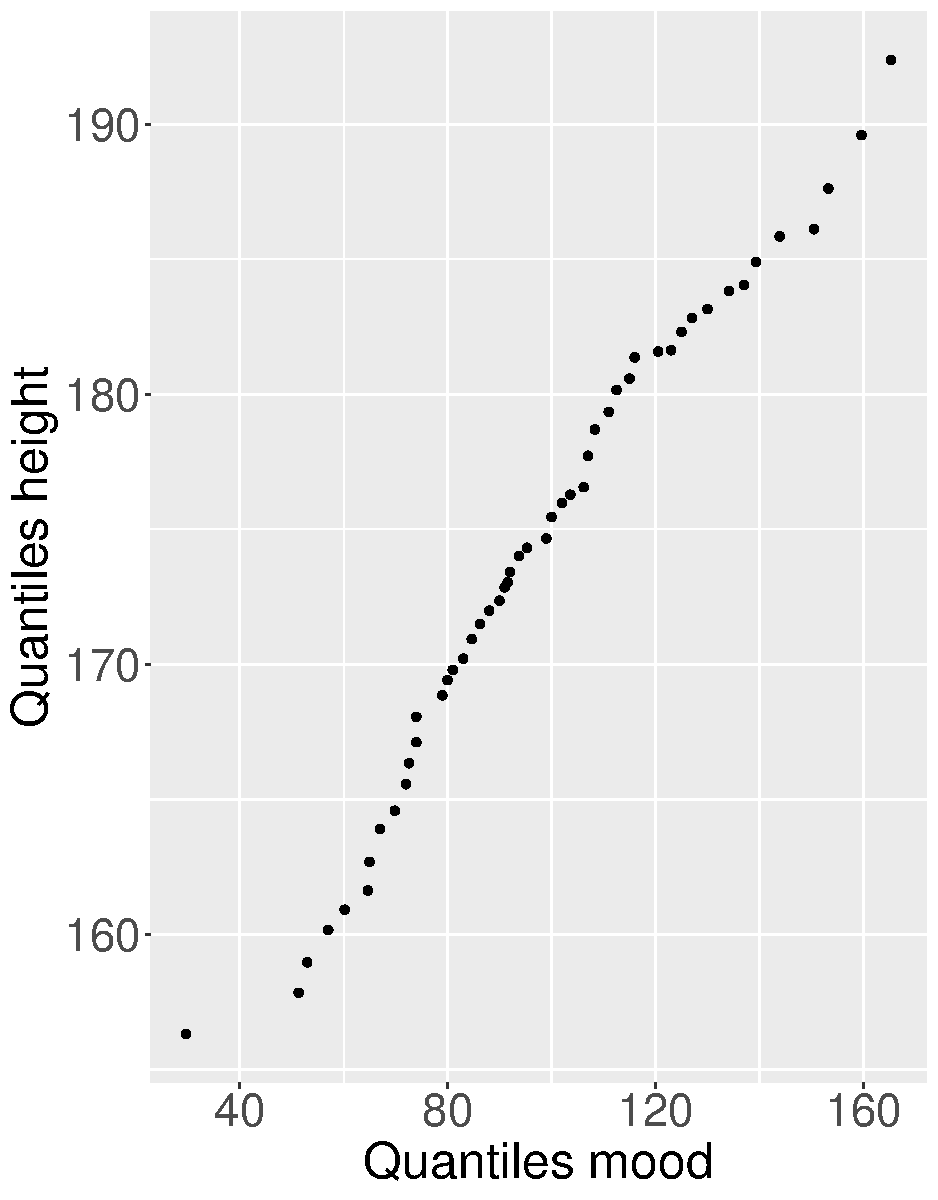
\includegraphics[width=6.25cm]{ggplot031b}
\vspace*{-0.5em}
\caption{Quantil-Quantil-Diagramme mit \lstinline!geom_qq()! und \lstinline!geom_qq_line()!}
\label{fig:ggplot031}
\end{figure}

%%%%%%%%%%%%%%%%%%%%%%%%%%%%%%%%%%%%%%%%%%%%%%%%%%%%%%%%%%%%%%%%%%
%%%%%%%%%%%%%%%%%%%%%%%%%%%%%%%%%%%%%%%%%%%%%%%%%%%%%%%%%%%%%%%%%%
\section{Bedingte Diagramme in Panels darstellen}
\label{sec:ggplotFacet}
%%%%%%%%%%%%%%%%%%%%%%%%%%%%%%%%%%%%%%%%%%%%%%%%%%%%%%%%%%%%%%%%%%
%%%%%%%%%%%%%%%%%%%%%%%%%%%%%%%%%%%%%%%%%%%%%%%%%%%%%%%%%%%%%%%%%%

\index{Grafik!bedingte Diagramme}

Multivariate Daten, deren Variablen teilweise kategorial sind, lassen sich durch bedingte Diagramme visualisieren: Dafür wird die gesamte Diagrammfläche in \emph{Facetten} (\emph{panels}) unterteilt und in den Facetten getrennt für jede Stufe einer kategorialen Variable derselbe Diagrammtyp dargestellt. Bei mehreren Faktoren ist dies für jede Kombination von Stufen verschiedener Faktoren möglich.

\begin{itemize}
\item Um die Diagrammregion in einzelne Facetten aufzuteilen, die jeweils einer Gruppe zugeordnet sind, kann eine mit \index[func]{facet_grid()@\lstinline{facet_grid()}} \lstinline!facet_grid(<<Zeilen>> ~ <<Spalten>>)! erstellte Schicht hinzugefügt werden. Dabei definiert die übergebene Modellformel die Aufteilung der Diagrammfläche jeweils in Zeilen und Spalten durch links und rechts der \lstinline!~! genannte Faktoren. Sollen Zeilen oder Spalten nicht unterteilt werden, ist statt eines Faktors ein \lstinline!.! zu nennen.
\item \index[func]{facet_wrap()@\lstinline{facet_wrap()}} \lstinline!facet_wrap(~ <<Faktor>>, nrow=<<Anzahl>>, ncol=<<Anzahl>>)! erstellt ebenfalls eine Facette für jede Gruppe des rechts der \lstinline!~! genannten Faktors, ordnet die Facetten aber selbständig in einer gekachelten Fläche an. Sollen die Gruppen aus der Kombination zweier Faktoren gebildet werden, kann die Formel \lstinline!~ <<Faktor1>> + <<Faktor2>>! lauten -- analog für weitere Faktoren. Die Anzahl der Zeilen und Spalten des Diagramms lässt sich durch \lstinline!nrow! und \lstinline!ncol! vorgeben.
\item In der Voreinstellung erhalten alle panels dieselben Achsenbereiche. Es ist jedoch möglich, mit dem Argument \lstinline!scales="free_y"! von \lstinline!facet_grid()! pro Zeile eine eigene $y$-Achse und mit \lstinline!scales="free_x"! pro Spalte eine eigene $x$-Achse zu definieren. \lstinline!scales="free"! kombiniert beide Optionen. Auch \lstinline!facet_wrap()! akzeptiert diese Optionen, gibt dann jedoch jeder Facette eine eigene $x$- bzw.\ $y$-Achse, also mehrere $y$-Achsen pro Zeile bzw.\ mehrere $x$-Achsen pro Spalte.
\end{itemize}

Zunächst sollen nach Geschlecht getrennte boxplots in separaten panels für die Gruppen dargestellt werden (Abb.\ \ref{fig:ggplot05}). Abschnitt \ref{sec:ggplotLegend} zeigt, wie die hier unnötige Legende entfernt werden kann.
\begin{lstlisting}
> ggplot(myDf, aes(x=sex, y=height, fill=sex)) +
+     geom_boxplot() +
+     facet_grid(. ~ group)
\end{lstlisting}

Nun soll für jede Kombination von Geschlecht und Gruppe jeweils ein panel das bedingte Streudiagramm von Körpergröße und Stimmung zeigen (Abb.\ \ref{fig:ggplot05}).
\begin{lstlisting}
> ggplot(myDf, aes(x=height, y=mood)) +
+     geom_point() +
+     facet_wrap(~ sex + group, ncol=2, scales="free_y")
\end{lstlisting}

\begin{figure}[ht]
\centering
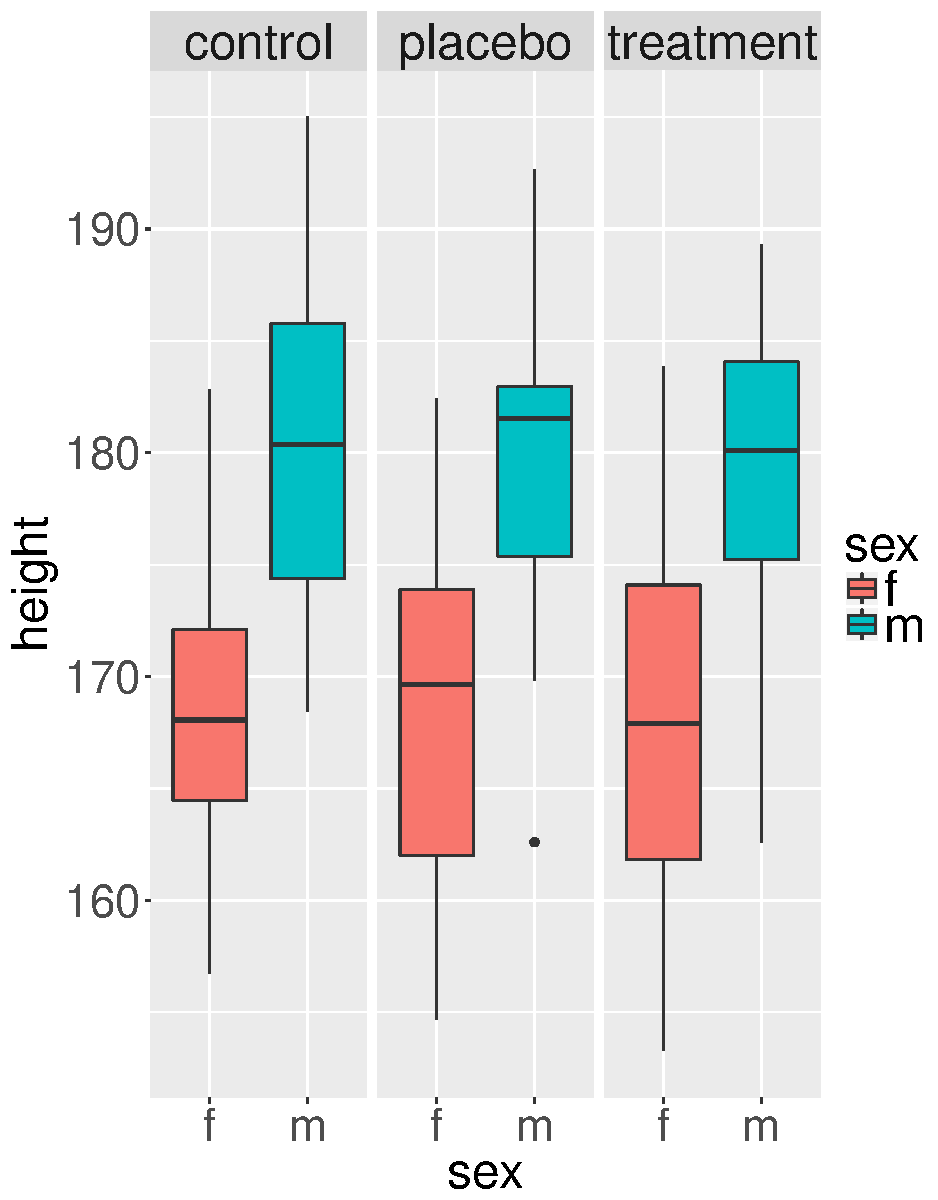
\includegraphics[width=6.25cm]{ggplot05a}
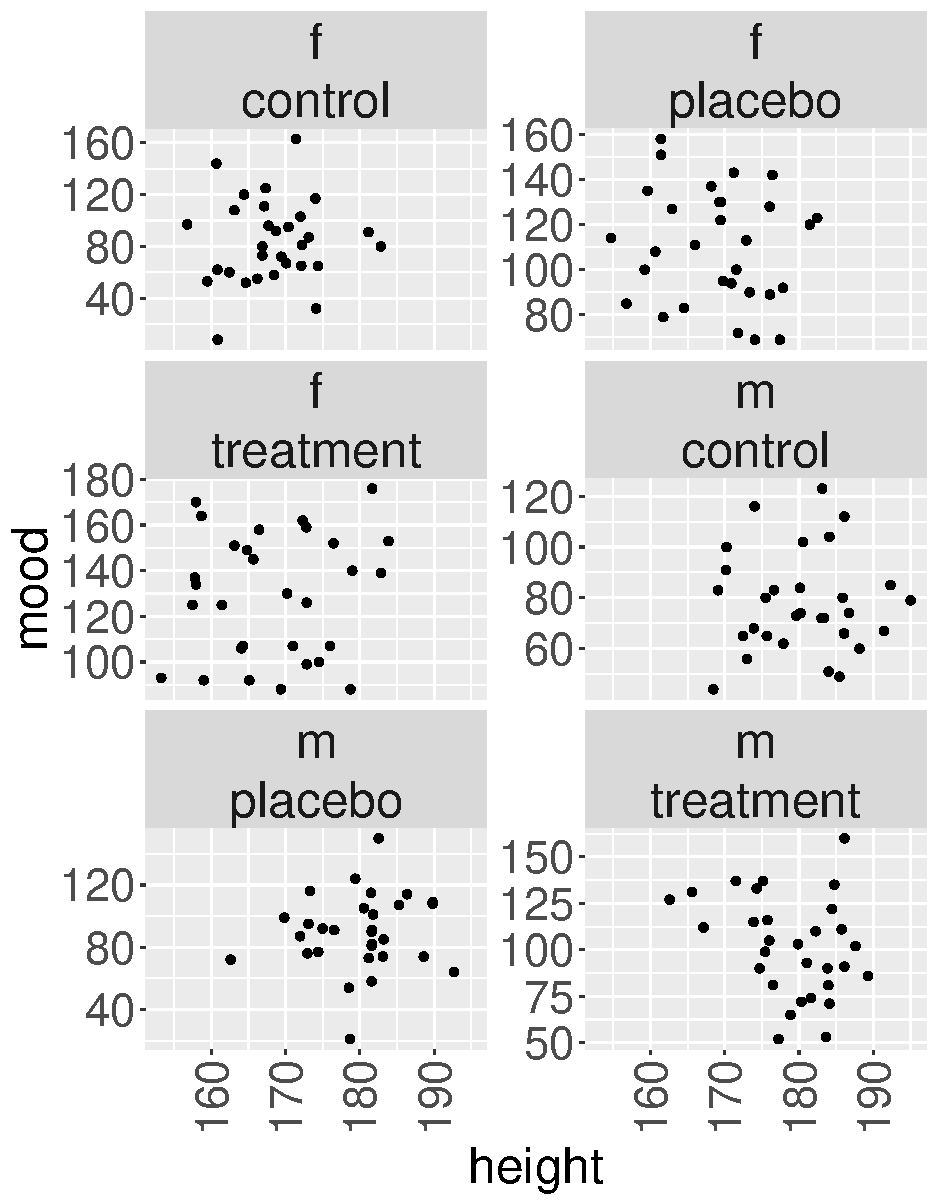
\includegraphics[width=6.25cm]{ggplot05b}
\vspace*{-0.5em}
\caption{Bedingte Diagramme in mehreren panels mit \lstinline!facet_grid()! und \lstinline!facet_wrap()!. Für senkrecht orientierte Beschriftungen der $x$-Achse s.\ Abschn.\ \ref{sec:ggplotAxis}.}
\label{fig:ggplot05}
\end{figure}

Analog zu den in Abschn.\ \ref{sec:diagSplit} vorgestellten Lösungen für Basis-Diagramme kann das Paket \index[pack]{patchwork@\lstinline{patchwork}} \lstinline!patchwork! \cite{Pedersen2019} verschiedene \lstinline!ggplot!-Objekte zu einem gemeinsamen Diagramm kombinieren. Dabei lässt sich die Aufteilung der Diagrammfläche sehr flexibel steuern. Auch ist es möglich, Teildiagramme mit Beschriftungen wie a) oder b) zu versehen und weiteren beliebigen Text auf dem Diagramm einzutragen.

%%%%%%%%%%%%%%%%%%%%%%%%%%%%%%%%%%%%%%%%%%%%%%%%%%%%%%%%%%%%%%%%%%
%%%%%%%%%%%%%%%%%%%%%%%%%%%%%%%%%%%%%%%%%%%%%%%%%%%%%%%%%%%%%%%%%%
\section{Diagrammelemente hinzufügen}
\label{sec:ggplotAddElem}
%%%%%%%%%%%%%%%%%%%%%%%%%%%%%%%%%%%%%%%%%%%%%%%%%%%%%%%%%%%%%%%%%%
%%%%%%%%%%%%%%%%%%%%%%%%%%%%%%%%%%%%%%%%%%%%%%%%%%%%%%%%%%%%%%%%%%

Einer Grundschicht mit konkretem Diagramm lassen sich mit \lstinline!+! weitere Schichten mit Diagrammelementen hinzufügen, etwa vertikale bzw.\ horizontale Linien oder Regressionsgeraden. Diese Elemente sind frei miteinander kombinierbar und können sich über die Argumente \lstinline!data! sowie \lstinline!aes()! der hinzufügenden Funktion ggf.\ auch auf andere Daten als die der Grundschicht beziehen.

Geometrische Grundformen:
\begin{itemize}
\item \index[func]{geom_segment()@\lstinline{geom_segment()}} \lstinline!geom_segment(x=<<Vektor>>, y=<<Vektor>>, xend=<<Vektor>>, yend=<<Vektor>>)! für Liniensegmente, die bei Koordinaten \lstinline!x!, \lstinline!y! beginnen und \lstinline!xend!, \lstinline!yend! enden. Über das Argument \lstinline!arrow! lassen sie sich auch als Pfeile zeichnen.
\item \index[func]{geom_polygon()@\lstinline{geom_polygon()}} \lstinline!geom_polygon()! für Polygone, wodurch man z.\,B.\ Umrisse in Karten zeichnen kann.
\item \index[func]{geom_rect()@\lstinline{geom_rect()}} \lstinline!geom_rect(xmin=<<Vektor>>, xmax=<<Vektor>>, ymin=<<Vektor>>, ymax=<<Vektor>>)! für Rechtecke, deren linke untere Ecke über Koordinaten \lstinline!xmin!, \lstinline!ymin! und deren rechte obere Ecke über \lstinline!xmax!, \lstinline!ymax! definiert ist.
\end{itemize}

Besondere Diagrammelemente:
\begin{itemize}
\item \index[func]{labs()@\lstinline{labs()}} \lstinline!labs(title="<<Text>>", subtitle="<<Text>>")! für einen Diagrammtitel und -untertitel.
\item \index[func]{geom_vline()@\lstinline{geom_vline()}} \lstinline!geom_vline(aes(xintercept=<<x-Koord.>>))! für vertikale Linien, die die $x$-Achse in \lstinline!xintercept! schneiden.
\item \index[func]{geom_hline()@\lstinline{geom_hline()}} \lstinline!geom_hline(aes(yintercept=<<y-Koord.>>))! für horizontale Linien, die die $y$-Achse in \lstinline!yintercept! schneiden.
\item \index[func]{geom_ribbon()@\lstinline{geom_ribbon()}} \lstinline!geom_ribbon()! für eine Fläche zwischen den im Aufruf von \lstinline!aes()! definierten $y$-Koordinaten \lstinline!ymin=<<untere Grenze>>! und \lstinline!ymax=<<obere Grenze>>!. Eine mögliche Anwendung ist die Darstellung eines durchgehenden Konfidenzbereichs um eine Vorhersage.
\item \index[func]{geom_linerange()@\lstinline{geom_linerange()}} \lstinline!geom_linerange()! für vertikale Liniensegmente, die im Aufruf von \lstinline!aes()! über die Argumente \lstinline!ymin=<<Vektor>>! und \lstinline!ymax=<<Vektor>>! definiert werden. Eine mögliche Anwendung ist die Darstellung von punktweisen Konfidenzintervallen.
\item \index[func]{geom_errorbar()@\lstinline{geom_errorbar()}} \lstinline!geom_errorbar()! für klassische Fehlerbalken, die im Aufruf von \lstinline!aes()! über die Argumente \lstinline!ymin=<<Vektor>>! und \lstinline!ymax=<<Vektor>>! definiert werden. Im Gegensatz zu \lstinline!geom_linerange()! besitzen sie Querlinien am oberen und unteren Ende des dargestellten Intervalls.
\item \index[func]{geom_rug()@\lstinline{geom_rug()}} \lstinline!geom_rug()! für eine Darstellung der Einzelwerte einer Verteilung als vertikale Striche entlang der $x$- oder $y$-Achse -- z.\,B.\ in Kombination mit einem Kerndichteschätzer.
\item \index[func]{geom_smooth()@\lstinline{geom_smooth()}} \lstinline!geom_smooth(method=<<Methode>>, se=TRUE, level=0.95, fullrange=FALSE)! für eine automatisch berechnete Regressionslinie. Dies ist etwa die Vorhersage einer linearen Regression mit \lstinline!method=lm! (Abschn.\ \ref{sec:regrSimple}) oder ein lokaler LOESS-Glätter mit \lstinline!method=loess! (Abschn.\ \ref{sec:loess}, Voreinstellung für kleinere Datensätze). Mit \lstinline!se=TRUE! erhält man zusätzlich den Konfidenzbereich für die Regressionslinie zum Niveau \lstinline!level!. Mit \lstinline!fullrange=TRUE! erstreckt sich die Regressionslinie bis an den Rand eines Diagramms, extrapoliert also über den beobachteten Wertebereich der $x$-Variable hinaus.
\item \index[func]{geom_text()@\lstinline{geom_text()}} \lstinline!geom_text(aes(x=<<x-Koord.>>, y=<<y-Koord.>>, label=<<Variable>>))! für Text, der in jeder Facette des Diagramms an den Koordinaten \lstinline!x! und \lstinline!y! erscheinen soll. Für \lstinline!label! ist die Variable des Datensatzes im Aufruf von \lstinline!ggplot()! zu nennen, die diesen Text für jede Beobachtung enthält.
\item \index[func]{annotate()@\lstinline{annotate()}} \lstinline!annotate("text", x=<<x-Koord.>>, y=<<y-Koord.>>, label="<<Anmerkung>>"))! für Textanmerkungen, die in jeder Facette des Diagramms identisch sind und an den Koordinaten \lstinline!x! und \lstinline!y! erscheinen sollen, wobei dieser Text an das Argument \lstinline!label! zu übergeben ist.
\end{itemize}

Der in Abschn.\ \ref{sec:ggplotPoint} erstellte Datensatz der Gruppenmittelwerte der Stimmung soll hier um die gruppenweise Streuung der Stimmung sowie um die jeweilige Zellbesetzung ergänzt werden. Die einzelnen Datensätze lassen sich mit \lstinline!merge()! (Abschn.\ \ref{sec:merge}) zu einem gemeinsamen Datensatz zusammenführen, dem der gruppenweise Standardfehler hinzugefügt wird.
\begin{lstlisting}
# einzelne Datensätze für Zellbesetzung und gruppenweise Streuung
> groupN  <- as.data.frame(xtabs(~ sex + group, data=myDf))
> groupSD <- aggregate(mood ~ sex + group, data=myDf, FUN=sd)

# führe einzelne Datensätze zusammen
> groupMSD   <- merge(groupM, groupSD, by=c("sex", "group"),
+                     suffixes=c(".M", ".SD"))

> groupMSDN  <- merge(groupMSD, groupN, by=c("sex", "group"))

# berechne Standardfehler
> (groupMSDN <- transform(groupMSDN,
+                         SEMlo=mood.M - mood.SD/sqrt(Freq),
+                         SEMup=mood.M + mood.SD/sqrt(Freq)))     # ...
\end{lstlisting}

Das in Abschn.\ \ref{sec:ggplotPoint} gezeigte Liniendiagramm der Gruppenmittelwerte soll nun mit Fehlerbalken erweitert werden, die $\pm 1$ Standardfehler darstellen (Abb.\ \ref{fig:ggplot6a}).
\begin{lstlisting}
> ggplot(groupMSDN,
+        aes(x=group, y=mood.M, ymin=SEMlo, ymax=SEMup,
+            color=sex, shape=sex, group=sex)) +
+     geom_point() +
+     geom_line() +
+     geom_linerange()
\end{lstlisting}

\begin{figure}[ht]
\centering
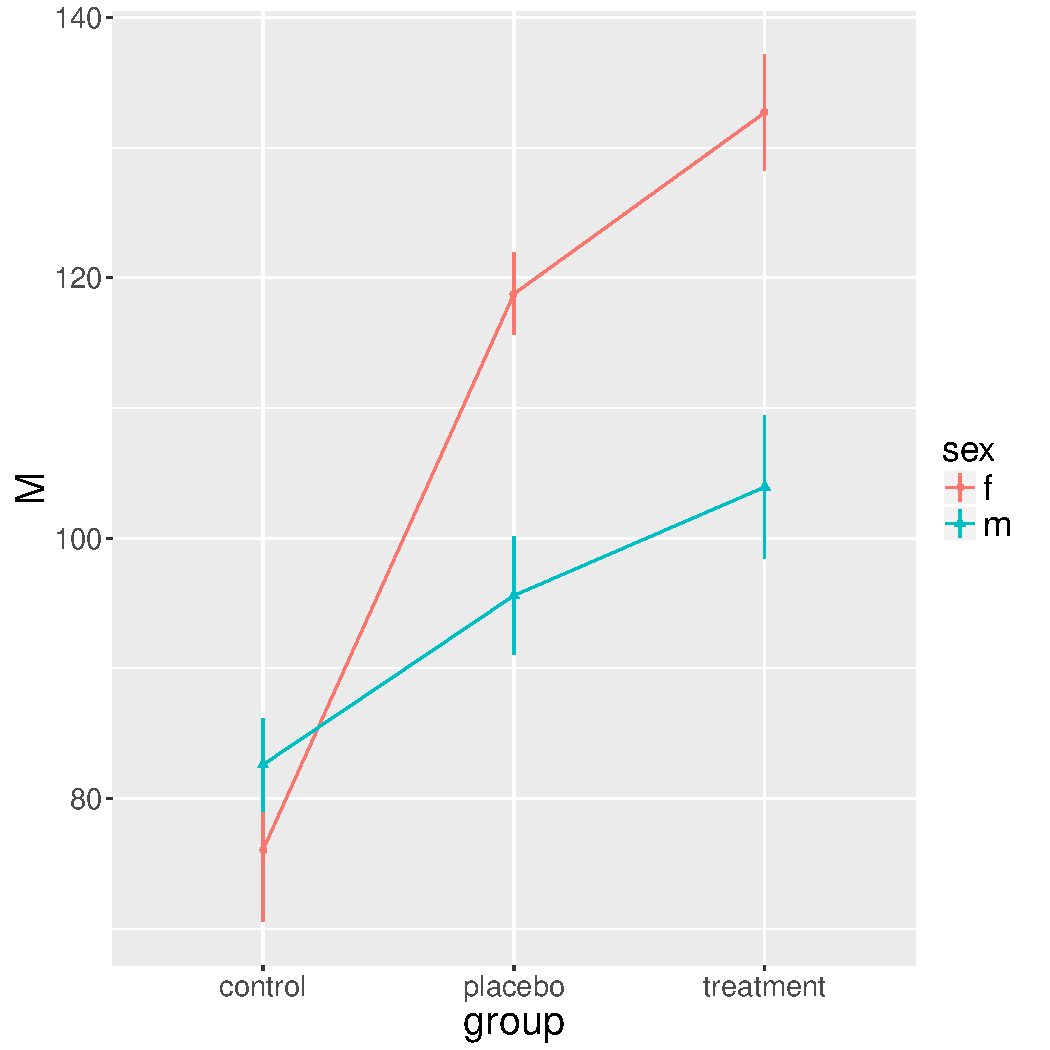
\includegraphics[width=8cm]{ggplot06a}
\vspace*{-0.5em}
\caption{Liniendiagramm mit \lstinline!geom_line()! und Fehlerbalken mit \lstinline!geom_linerange()!}
\label{fig:ggplot6a}
\end{figure}

Abbildung \ref{fig:ggplot06b} soll nach Gruppen getrennte Streudiagramme inkl.\ Regressionsgerade samt Konfidenzbereich, horizontale wie vertikale Referenz-Linien sowie Text-labels in einem multi-panel layout kombinieren.
\begin{lstlisting}
> ggplot(myDf, aes(x=height, y=mood, colour=sex:group, shape=sex)) +
+     geom_hline(aes(yintercept=100), linetype=2) +
+     geom_vline(aes(xintercept=180), linetype=2) +
+     geom_point(size=3) +
+     geom_smooth(method=lm, se=TRUE, size=1.2, fullrange=TRUE) +
+     facet_grid(sex ~ group) +
+     labs(title="mood ~ height getrennt nach Geschlecht + Gruppe") +
+     geom_text(aes(x=190, y=70, label=sgComb)) +
+     annotate("text", x=165, y=5, label="Annotation")
\end{lstlisting}

\begin{figure}[ht]
\centering
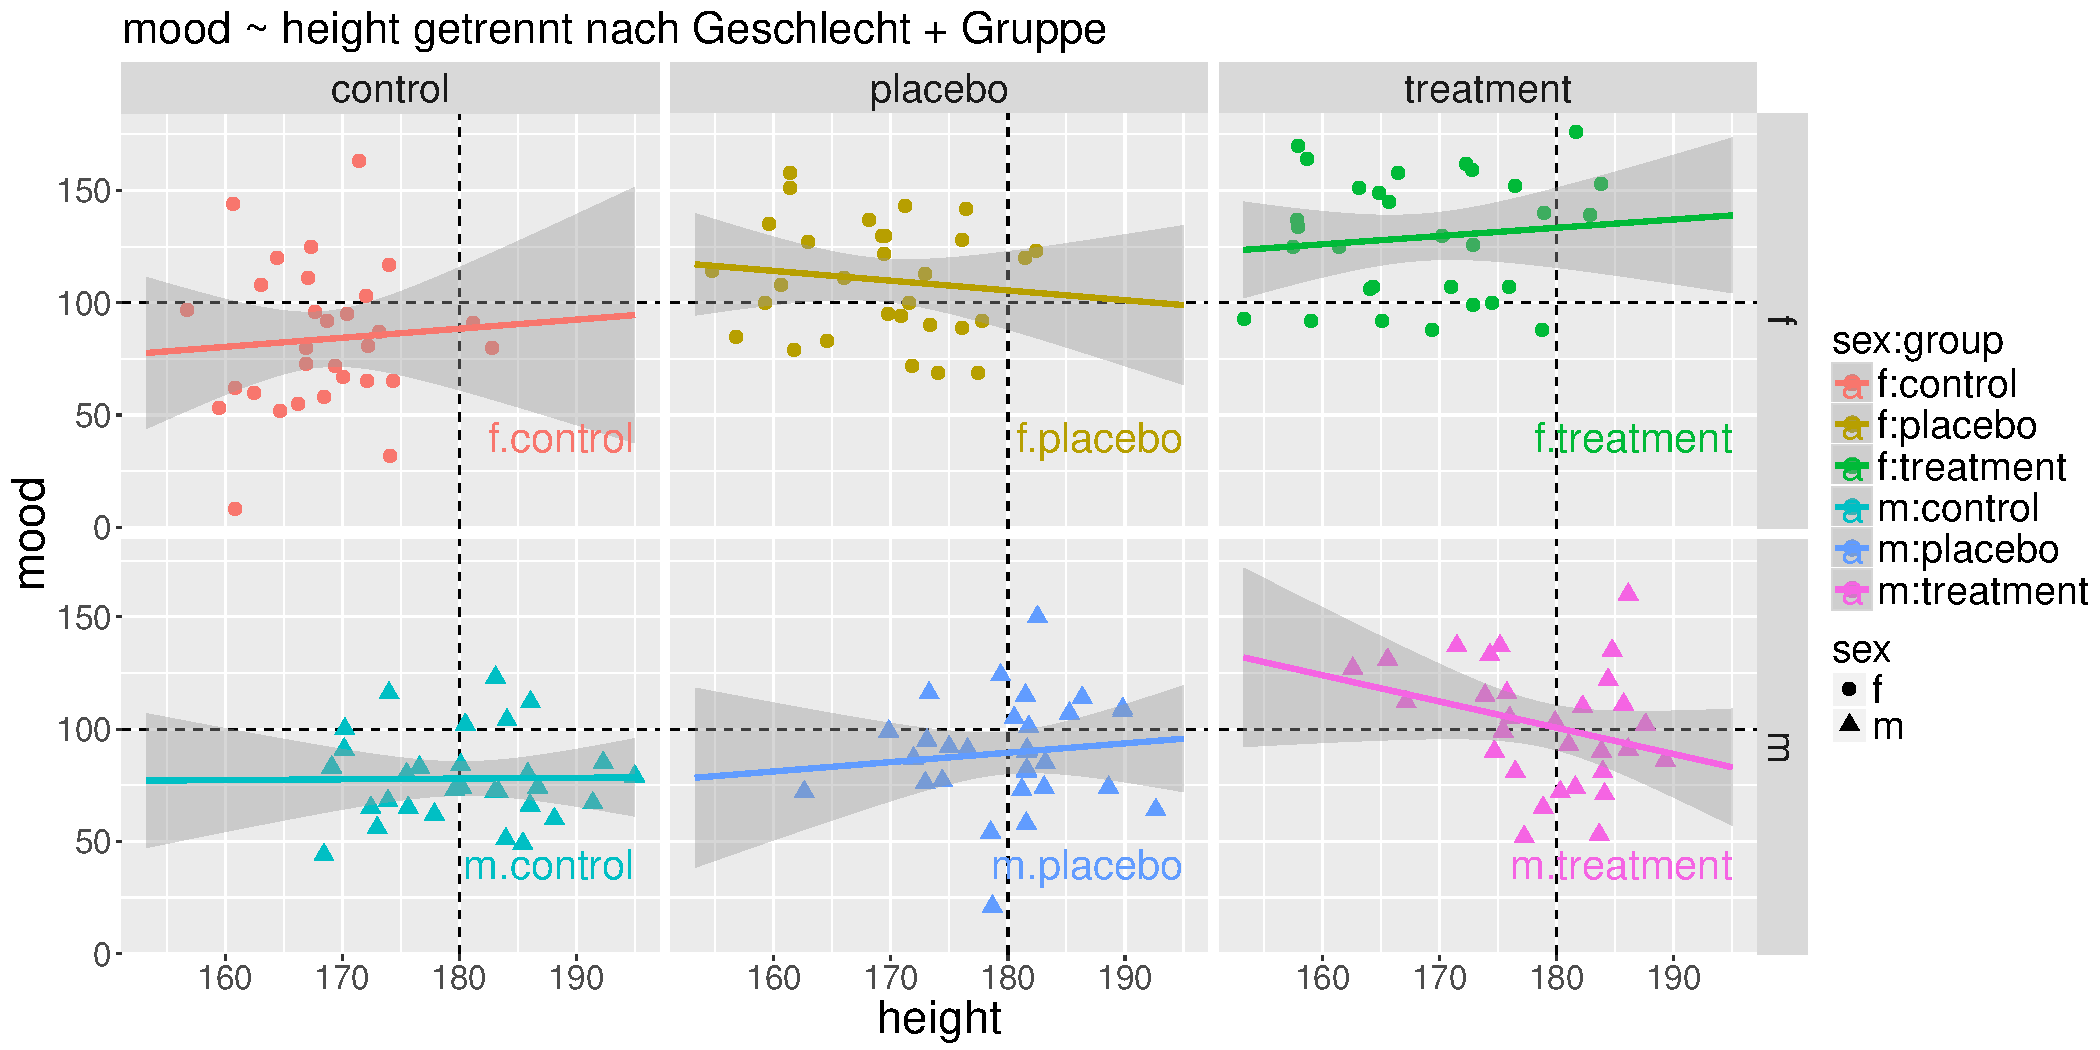
\includegraphics[width=12.5cm]{ggplot06b}
\vspace*{-0.5em}
\caption{Nach Gruppen getrennte Streudiagramme inkl.\ Regressionsgerade samt Konfidenzbereich mit \lstinline!geom_smooth()! sowie Text-labels mit \lstinline!geom_text()! und \lstinline!annotate()!}
\label{fig:ggplot06b}
\end{figure}

%%%%%%%%%%%%%%%%%%%%%%%%%%%%%%%%%%%%%%%%%%%%%%%%%%%%%%%%%%%%%%%%%%
%%%%%%%%%%%%%%%%%%%%%%%%%%%%%%%%%%%%%%%%%%%%%%%%%%%%%%%%%%%%%%%%%%
\section{Diagramme formatieren}
\label{sec:ggplotFormat}
%%%%%%%%%%%%%%%%%%%%%%%%%%%%%%%%%%%%%%%%%%%%%%%%%%%%%%%%%%%%%%%%%%
%%%%%%%%%%%%%%%%%%%%%%%%%%%%%%%%%%%%%%%%%%%%%%%%%%%%%%%%%%%%%%%%%%

Das Aussehen von \lstinline!ggplot2!-Diagrammen lässt sich über eine Vielzahl weiterer Argumente im Detail anpassen. Die wichtigsten Möglichkeiten zur individuellen Gestaltung werden im Folgenden vorgestellt.

%%%%%%%%%%%%%%%%%%%%%%%%%%%%%%%%%%%%%%%%%%%%%%%%%%%%%%%%%%%%%%%%%%
%%%%%%%%%%%%%%%%%%%%%%%%%%%%%%%%%%%%%%%%%%%%%%%%%%%%%%%%%%%%%%%%%%
\subsection{Elementposition kontrollieren}
\label{sec:ggplotPos}
%%%%%%%%%%%%%%%%%%%%%%%%%%%%%%%%%%%%%%%%%%%%%%%%%%%%%%%%%%%%%%%%%%
%%%%%%%%%%%%%%%%%%%%%%%%%%%%%%%%%%%%%%%%%%%%%%%%%%%%%%%%%%%%%%%%%%

Bei gruppiert dargestellten Daten mit kategorialer $x$-Achse zeigt das Diagramm für jede Kategorie der $x$-Achse mehrere Elemente -- z.\,B.\ boxplots oder Säulen. Diese Elemente lassen sich jeweils relativ zueinander auf verschiedene Arten anordnen. Dazu können die folgenden Funktionsaufrufe an das Argument \lstinline!position! von \lstinline!geom_<<Name>>()! Funktionen übergeben werden:
\begin{itemize}
\item \index[func]{position_stack()@\lstinline{position_stack()}} \lstinline!position_stack()! sorgt bei Säulendiagrammen dafür, dass die zu den Gruppen gehörenden Segmente aufeinander gestapelt werden (gestapeltes Säulendiagramm).
\item \index[func]{position_fill()@\lstinline{position_fill()}} \lstinline!position_fill()! stapelt ebenfalls die Segmente aufeinander, skaliert jedoch alle Gesamtsäulen auf dieselbe Höhe. Diese Anordnung ist etwa für die Präsentation bedingter relativer Häufigkeiten geeignet, die sich pro Kategorie der $x$-Achse zu 1 addieren.
\item \index[func]{position_dodge()@\lstinline{position_dodge()}} \lstinline!position_dodge(width=<<Breite>>)! ordnet Säulen oder boxplots nebeneinander an, kann also etwa ein gruppiertes Säulendiagramm erzeugen. Über \lstinline!width! lässt sich eine Lücke zwischen Diagrammelementen herstellen.
\item Überlappen sich bei eigentlich stetigen $x$- oder $y$-Koordinaten viele mit \lstinline!geom_point()! dargestellte Datenpunkte, kann man von der präzisen Positionierung abweichen, um alle Datenpunkte sichtbar zu machen: Übergibt man an das \lstinline!position! Argument \index[func]{position_jitter()@\lstinline{position_jitter()}}\\
\lstinline!position_jitter(width=<<Streubreite>>, height=<<Streubreite>>)!\\
sorgt dies dafür, dass $x$- oder $y$-Koordinaten mit einem kleinen zufälligen Versatz dargestellt werden. Die erzeugte halbe Streubreite legen \lstinline!width! bzw.\ \lstinline!height! fest -- Voreinstellung ist 0.4. Bei sehr vielen Datenpunkten ist u.\,U.\ die Kombination mit simulierter Transparenz sinnvoll, die das Argument \lstinline!alpha! von \lstinline!geom_<<Name>>()! Funktionen kontrolliert (Abschn.\ \ref{sec:ggplotColour}). Alternativ kann auf einen 2D-Dichteschätzer mit\index[func]{geom_hex()@\lstinline{geom_hex()}} \lstinline!geom_hex()! analog zu \lstinline!hexbin()! (Abschn.\ \ref{sec:distr2var}) ausgewichen werden.
\end{itemize}

Nach Gruppen getrennte Histogramme sollen zunächst versetzt nebeneinander dargestellt werden (Abb.\ \ref{fig:ggplot07}).
\begin{lstlisting}
> ggplot(myDf, aes(x=mood, fill=sex)) +
+     geom_histogram(aes(y=..density..),
+                    position=position_dodge())
\end{lstlisting}

Das folgende Diagramm stellt die bedingten relativen Häufigkeiten einer kategorialen Variable für verschiedene Gruppen in einem normierten Säulendiagramm dar (Abb.\ \ref{fig:ggplot07}). Abschnitt \ref{sec:ggplotAxis} zeigt, wie die hier nicht sinnvollen Achsenbeschriftungen angepasst werden können.
\begin{lstlisting}
> ggplot(myDf, aes(x=rating, group=sex, fill=sex)) +
+     geom_bar(stat="count",
+              aes(y=(..count..) / sum(..count..)),
+              position=position_fill())
\end{lstlisting}

\begin{figure}[ht]
\centering
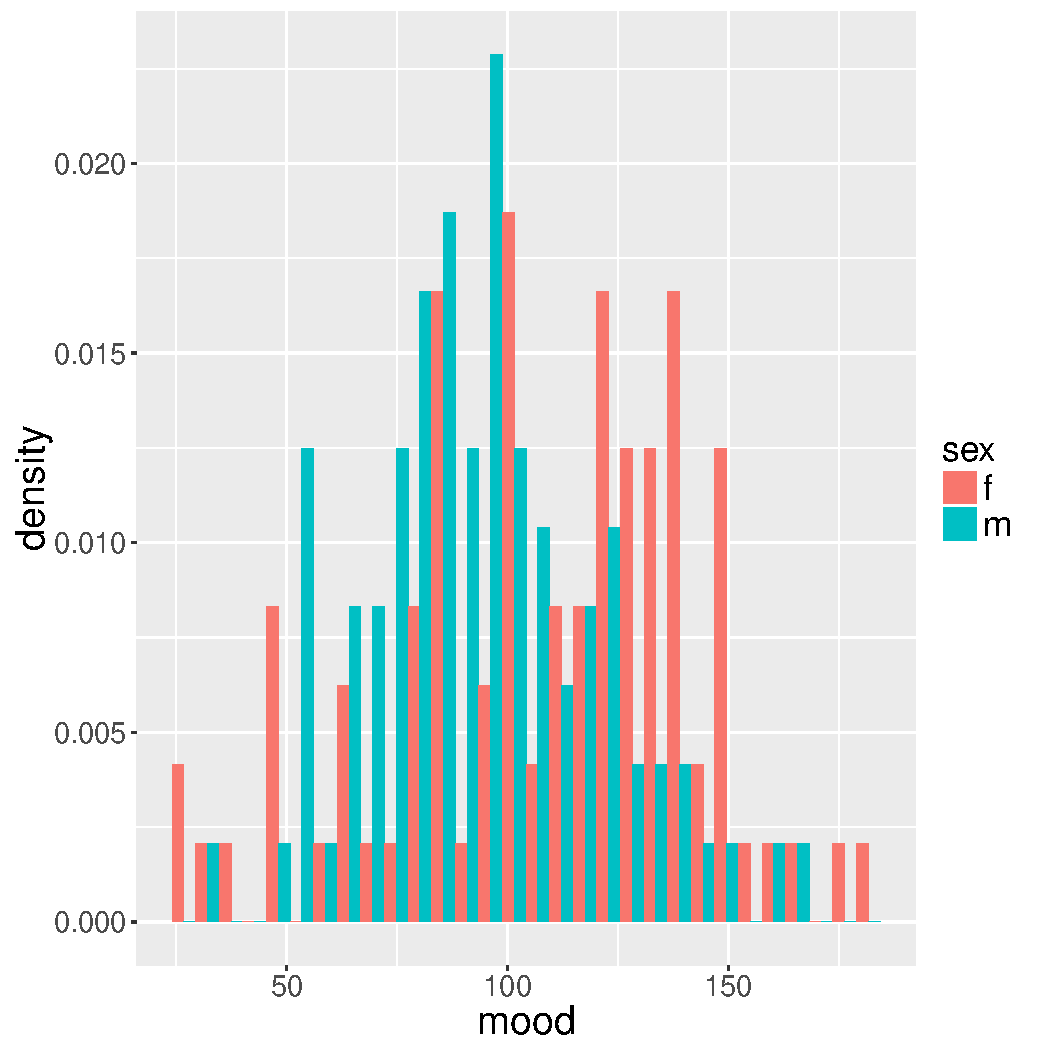
\includegraphics[width=6.25cm]{ggplot07a}
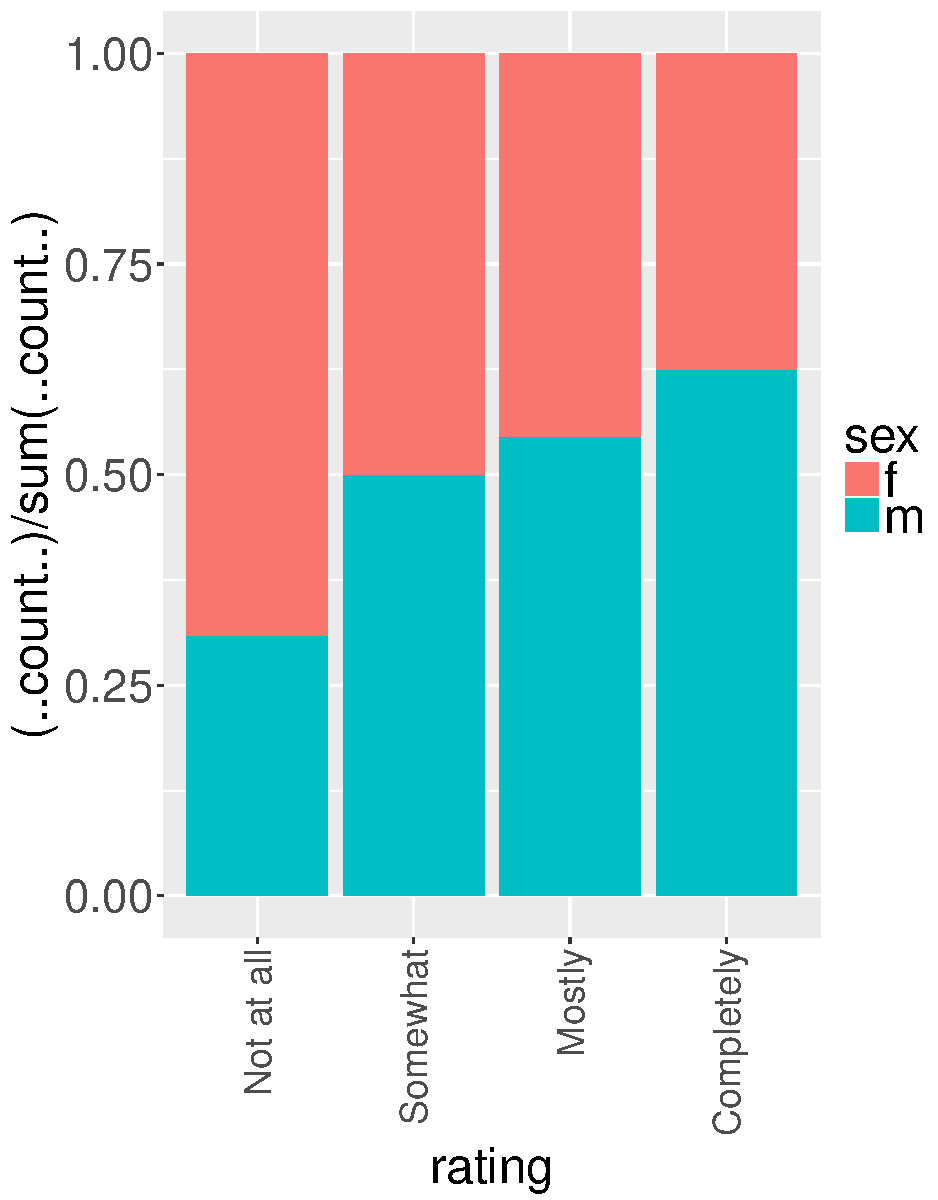
\includegraphics[width=6.25cm]{ggplot07b}
\vspace*{-0.5em}
\caption{Versetzte gruppenweise Histogramme mit \lstinline!position_dodge()! und gestapeltes normiertes Säulendiagramm mit \lstinline!position_fill()!. Für senkrecht orientierte Beschriftungen der $x$-Achse s.\ Abschn.\ \ref{sec:ggplotAxis}.}
\label{fig:ggplot07}
\end{figure}

%%%%%%%%%%%%%%%%%%%%%%%%%%%%%%%%%%%%%%%%%%%%%%%%%%%%%%%%%%%%%%%%%%
%%%%%%%%%%%%%%%%%%%%%%%%%%%%%%%%%%%%%%%%%%%%%%%%%%%%%%%%%%%%%%%%%%
\subsection{Achsen anpassen}
\label{sec:ggplotAxis}
%%%%%%%%%%%%%%%%%%%%%%%%%%%%%%%%%%%%%%%%%%%%%%%%%%%%%%%%%%%%%%%%%%
%%%%%%%%%%%%%%%%%%%%%%%%%%%%%%%%%%%%%%%%%%%%%%%%%%%%%%%%%%%%%%%%%%

Die folgenden Funktionen legen Skalierung, Wertebereich und genaue Position der Wertemarkierungen der Diagrammachsen fest, wenn sie mit \lstinline!+! einer Grundschicht hinzugefügt werden.

\begin{itemize}
\item \index[func]{labs()@\lstinline{labs()}} \lstinline!labs(x=<<"Text">>, y=<<"Text">>)! für Titel der $x$- und $y$-Achse.
\item \lstinline!guides(x=guide_axis(angle=90)))! sorgt für vertikal orientierte Wertebeschriftungen der $x$-Achse. Auch beliebige andere Winkel können für \lstinline!angle! angegeben werden. Analog lässt sich die Ausrichtung der Wertebeschriftungen der $y$-Achse mit dem Argument \lstinline!y! ändern.
\item \lstinline!theme(axis.ticks=element_blank()! entfernt die Wertmarkierungen der Achsen, \lstinline!theme(axis.text.x=element_blank())! löscht die Beschriftung der Wertmarkierungen der $x$-Achse.
%\item \index[func]{scale_x_discrete()@\lstinline{scale_x_discrete()}} \lstinline!scale_x_discrete(breaks=<<Vektor>>)! kontrolliert das Aussehen der $x$-Achse, wenn dort Werte einer kategorialen Variable dargestellt sind. Ein für \lstinline!breaks! angegebener Vektor von Kategorienbezeichnungen legt fest, welche Kategorien des mit der $x$-Achse verknüpften Faktors in welcher Reihenfolge dargestellt werden. In der Voreinstellung ist dies die Reihenfolge der Faktorstufen, also meist die alphabetische Reihenfolge (Abschn.\ \ref{sec:facLabelOrder}).
\item \index[func]{scale_x_date()@\lstinline{scale_x_date()}} \lstinline!scale_x_date(date_labels="<<Format-String>>")! bestimmt das Aussehen der $x$-Achse, wenn dort Werte einer Datumsvariable dargestellt sind. Insbesondere lässt sich die Formatierung des Datums mit einem Format-String für \lstinline!date_labels! festlegen, der wie in \lstinline!strptime()! aufgebaut ist (Abschn.\ \ref{sec:dateFormat}).
\item \index[func]{scale_x_continuous()@\lstinline{scale_x_continuous()}} \lstinline!scale_x_continuous()! definiert das Aussehen der $x$-Achse, wenn dort Werte einer stetigen Variable dargestellt sind. Insbesondere beschränkt ein für das Argument \lstinline!limits! angegebener Vektor den dargestellten Wertebereich. Die nicht in diesem Bereich liegenden Daten werden in allen weiteren Schichten nicht verwendet, etwa zur Definition von boxplots oder Regressionsgeraden (\emph{clipping}). Tatsächlich geht der dargestellte Wertebereich zu beiden Seiten etwas über die in \lstinline!limits! genannten Werte hinaus. Um die Achsen exakt bei diesen Werten enden zu lassen, kann \lstinline!expand=c(0, 0)! gesetzt werden. Die Anzahl der automatisch gesetzten Wertemarkierungen orientiert sich an der für \lstinline!n.breaks! genannten Anzahl. Ein für \lstinline!breaks! übergebener Vektor definiert zusätzlich, an welchen Stellen sich Wertemarkierungen befinden. Mit \lstinline!position="top"! wird die $x$-Achse am oberen Diagrammrand gezeichnet.
\item Bei einer kategorialen $x$-Achse ist die Reihenfolge der Einträge gleich der Reihenfolge der Stufen der dargestellten Variable, die dafür automatisch in einen Faktor umgewandelt wird. Die Reihenfolge lässt sich deswegen durch Anpassen dieses Faktors (Abschn.\ \ref{sec:facOrder}) vor Diagrammerstellung verändern. %, oder nur innerhalb der Legende mit \lstinline!scale_<<Eigenschaft>>_discrete(breaks=c("<<Stufe1>>", "<<Stufe2>>", ...))!, etwa \lstinline!scale_fill_discrete()! für die Füllfarbe von Flächen.
\item \index[func]{coord_cartesian()@\lstinline{coord_cartesian()}} \lstinline!coord_cartesian(xlim=<<Vektor>>, ylim=<<Vektor>>)! definiert den sichtbaren Wertebereich über die Argumente \lstinline!xlim! und \lstinline!ylim!. Im Unterschied zu \lstinline!scale_x_continuous()! werden die Datenpunkte dabei nicht von späteren Schichten ausgeschlossen, es wird also ohne \emph{clipping} gezoomt.
\item \index[func]{coord_fixed()@\lstinline{coord_fixed()}} \lstinline!coord_fixed(ratio=<<Zahl>>)! definiert das Längenverhältnis einer Einheit der $x$-Achse zu einer Einheit der $y$-Achse. Gleich skalierte Achsen erhält man mit \lstinline!ratio=1!.
\item \index[func]{coord_flip()@\lstinline{coord_flip()}} \lstinline!coord_flip(xlim=<<Vektor>>, ylim=<<Vektor>>)! vertauscht die Rolle von $x$- und $y$-Achse. Vertikale Linien parallel zur $y$-Achse werden so zu horizontalen Linien parallel zur $x$-Achse, etc. Sollen die dargestellten Wertebereiche dabei geändert werden, muss dies innerhalb von \lstinline!coord_flip()! über die Argumente \lstinline!xlim! und \lstinline!ylim! geschehen.
\end{itemize}

Alle \lstinline!scale_x_<<Name>>()! Funktionen haben ein Pendant für die $y$-Achse, das entsprechend \lstinline!scale_y_<<Name>>()! heißt.

Achsen können mit folgender Schicht auch als Pfeile gezeichnet werden:
\begin{lstlisting}
> theme(axis.line=element_line(arrow=arrow(length=unit(0.4, "cm"),
+                                          type="closed")))
\end{lstlisting}

Das folgende Diagramm zeigt geänderte Achsentitel, eine modifizierte Reihenfolge der $x$-Achsen Kategorien sowie senkrecht orientierte Wertebeschriftungen der $x$-Achse (Abb.\ \ref{fig:ggplot08a}).
\begin{lstlisting}
> levels(myDf$rating)     # aktuelle Reihenfolge der Stufen
[1] "Completely" "Mostly" "Somewhat" "Not at all"

# umgekehrte Reihenfolge der Stufen
> levels(myDf$rating) <- rev(levels(myDf$rating))
> ggplot(myDf, aes(x=rating, group=sex, fill=sex)) +
+     geom_bar(stat="count",
+              aes(y=(..count..) / sum(..count..)),
+              position=position_fill()) +
+     labs(x="Rating category", y="Cumulative relative frequency") +
+     guides(x=guide_axis(angle=90)
\end{lstlisting}

\begin{figure}[ht]
\centering
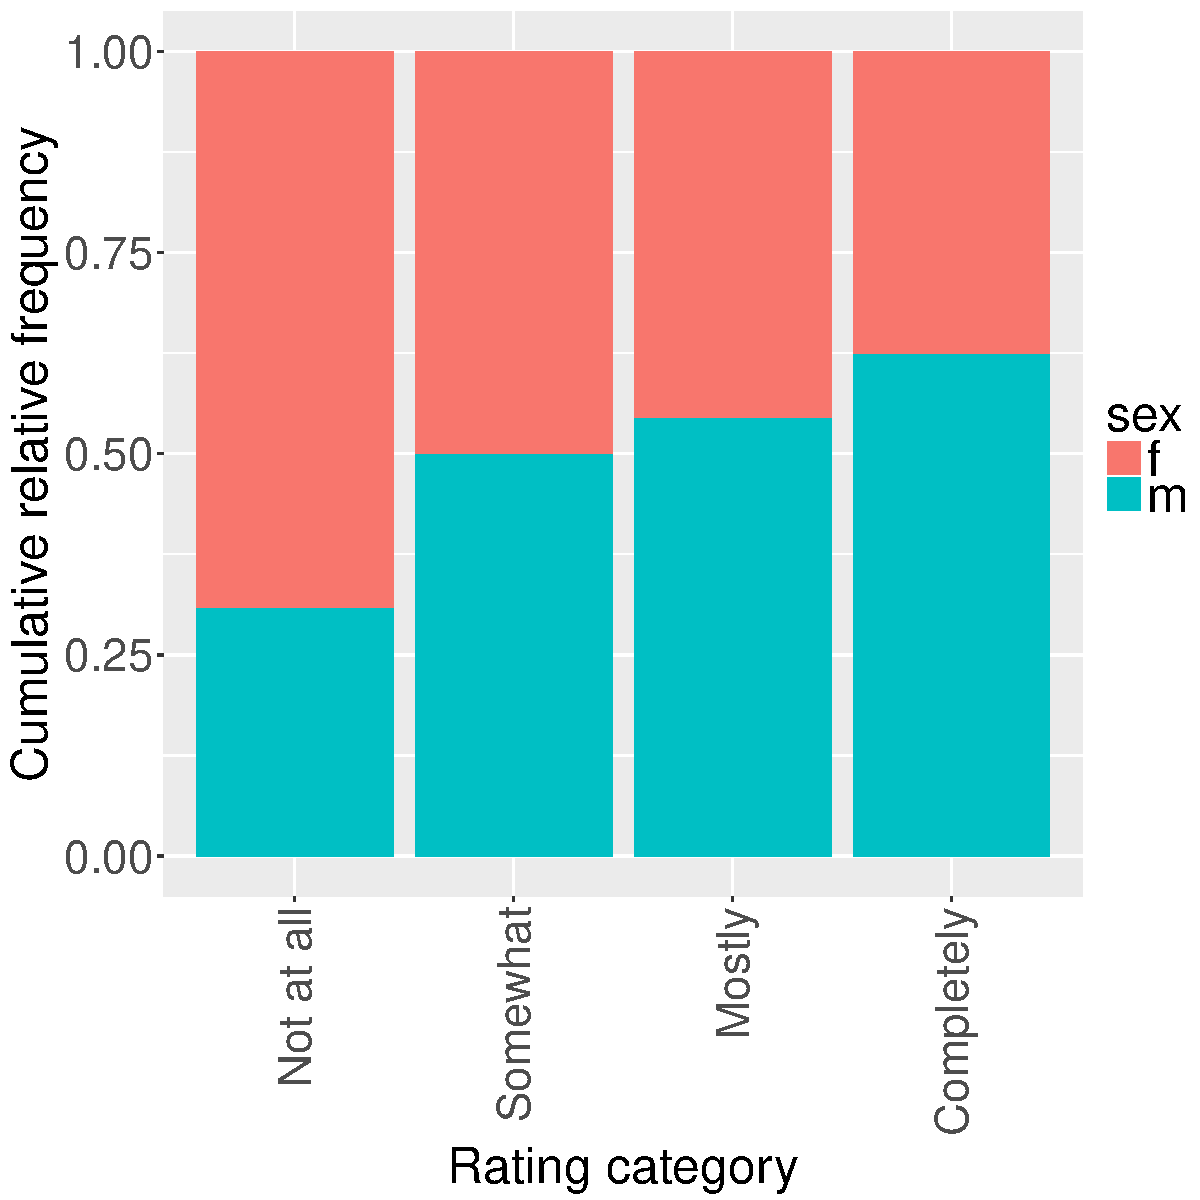
\includegraphics[width=8cm]{ggplot08a}
\vspace*{-0.5em}
\caption{Angepasste Achseneigenschaften mit \lstinline!scale_x_discrete()!, \lstinline!labs()! und \lstinline!guides()!}
\label{fig:ggplot08a}
\end{figure}

Das folgende Streudiagramm passt die Gitterabstände für $x$- und $y$-Achse an und verwendet senkrecht orientierte Wertebeschriftungen der $x$-Achse  (Abb.\ \ref{fig:ggplot08bc}).
\begin{lstlisting}
> ggplot(myDf, aes(x=height, y=mood, colour=sex, shape=group)) +
+     geom_point(size=3) +
+     scale_x_continuous(limits=c(150, 200),
+                        expand=c(0, 0),
+                        breaks=seq(150, 200, by=5)) +
+     scale_y_continuous(n.breaks=8) +
+     guides(x=guide_axis(angle=90))
\end{lstlisting}

Das folgende Diagramm vertauscht die Rolle von $x$- und $y$-Achse (Abb.\ \ref{fig:ggplot08bc}).
\begin{lstlisting}
> ggplot(myDf, aes(x=sex, y=height, fill=sex)) +
+     geom_boxplot() +
+     coord_flip(ylim=c(140, 200))
\end{lstlisting}

\begin{figure}[ht]
\centering
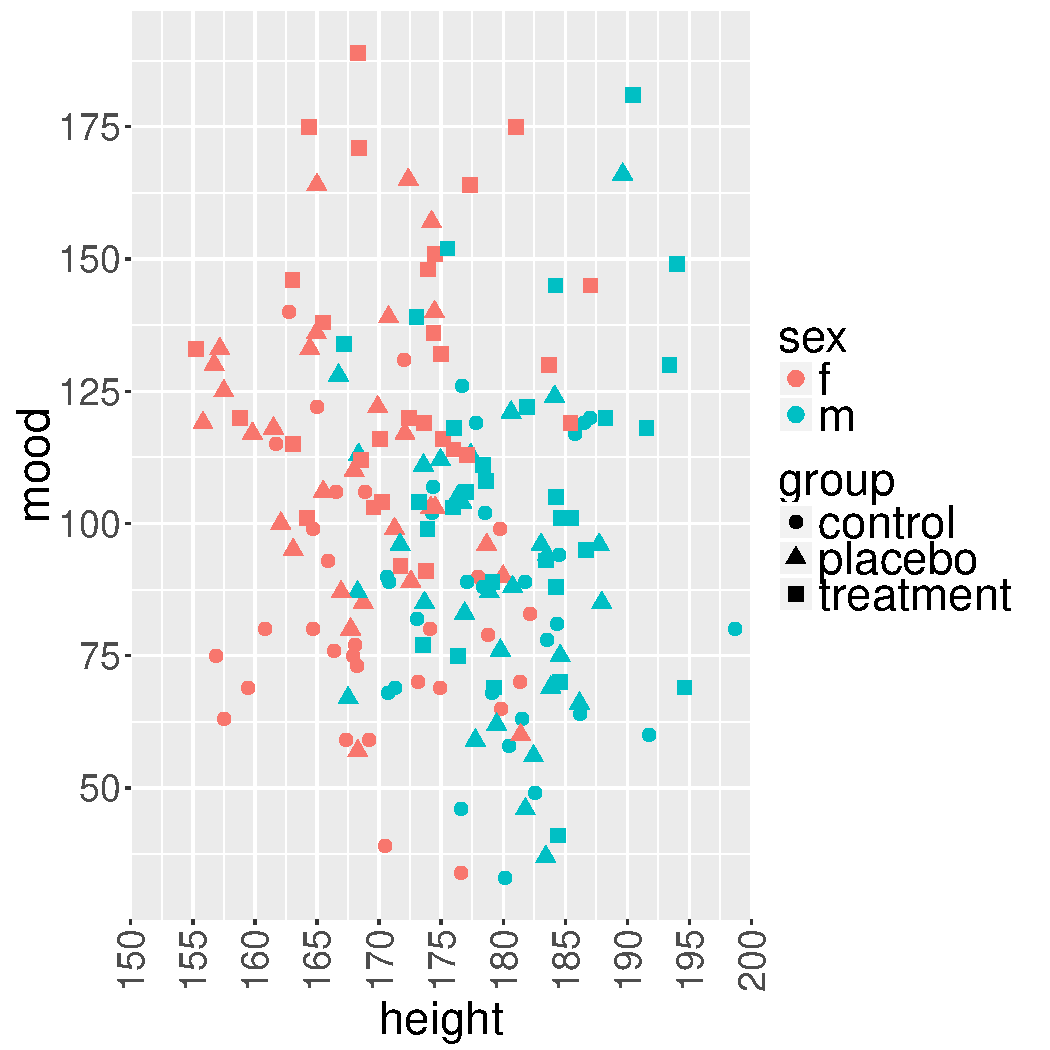
\includegraphics[width=6.25cm]{ggplot08b}
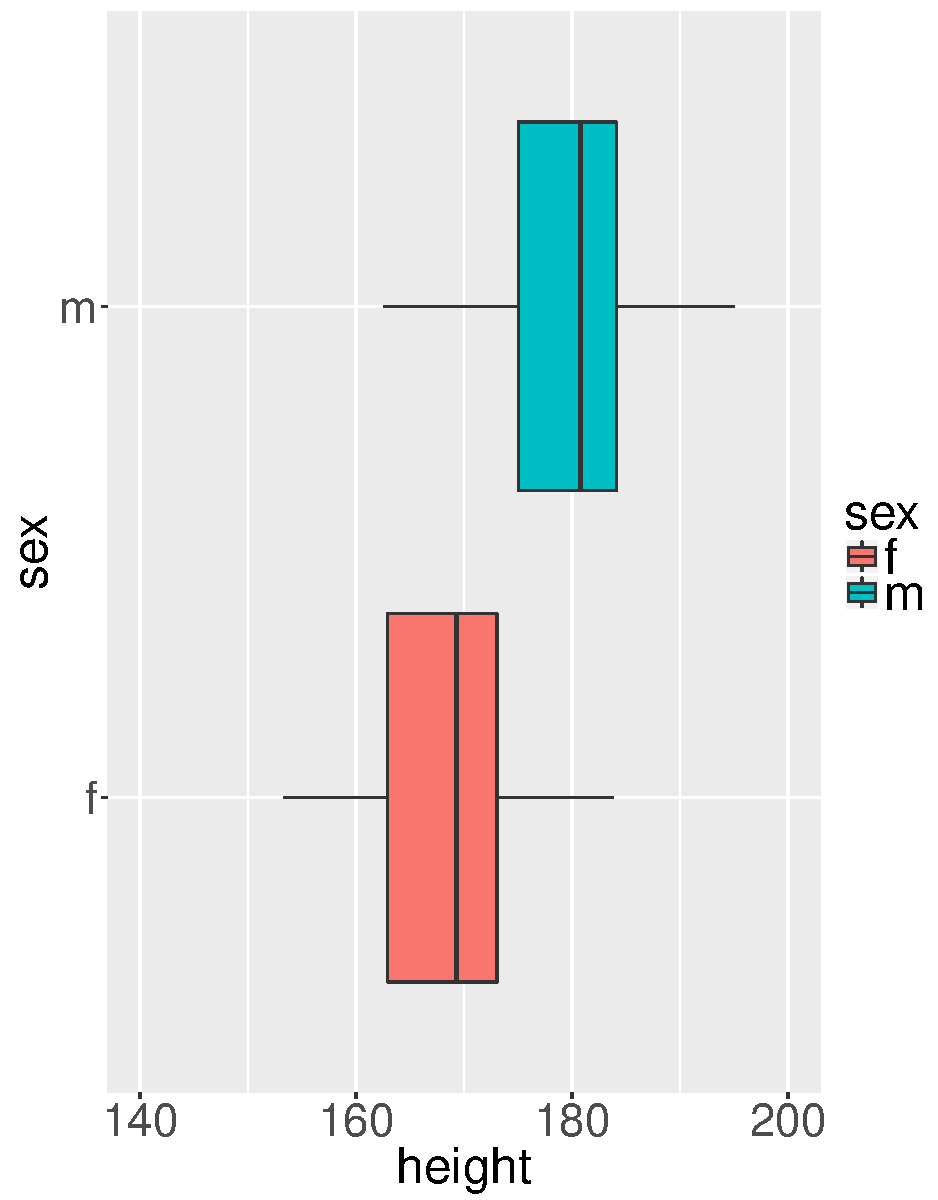
\includegraphics[width=6.25cm]{ggplot08c}
\vspace*{-0.5em}
\caption{Angepasste Achseneigenschaften mit \lstinline!scale_x_continuous()!, \lstinline!theme()! und \lstinline!coord_flip()!}
\label{fig:ggplot08bc}
\end{figure}

%%%%%%%%%%%%%%%%%%%%%%%%%%%%%%%%%%%%%%%%%%%%%%%%%%%%%%%%%%%%%%%%%%
%%%%%%%%%%%%%%%%%%%%%%%%%%%%%%%%%%%%%%%%%%%%%%%%%%%%%%%%%%%%%%%%%%
\subsection{Legende ändern}
\label{sec:ggplotLegend}
%%%%%%%%%%%%%%%%%%%%%%%%%%%%%%%%%%%%%%%%%%%%%%%%%%%%%%%%%%%%%%%%%%
%%%%%%%%%%%%%%%%%%%%%%%%%%%%%%%%%%%%%%%%%%%%%%%%%%%%%%%%%%%%%%%%%%

Die automatisch dargestellte Legende lässt sich in vielen Details an eigene Vorstellungen anpassen.

\begin{itemize}
\item \lstinline!theme(legend.position="none")! sorgt dafür, dass das Diagramm keine Legende zeigt. Um dagegen die Legende an verschiedenen Stellen zu positionieren, kann \lstinline!legend.position! auf \lstinline!"left"!, \lstinline!"right"!, \lstinline!"bottom"!, \lstinline!"top"! oder auf einen Vektor von relativen $(x,y)$-Koordinaten im Bereich 0--1 gesetzt werden.
\item \index[func]{guides()@\lstinline{guides()}} \lstinline!guides(<<Eigenschaft>>=FALSE)! entfernt aus der Legende das zu \lstinline!<<Eigenschaft>>! gehörende Element. So sorgt etwa \lstinline!shape=FALSE! dafür, dass die Legende keine Einträge zur Art der verwendeten Datenpunktsymbole enthält.
\item \lstinline!guides(<<Eigenschaft>>=guide_legend(title=NULL))! bewirkt, dass die eine bestimmte Eigenschaft erklärende Legende keinen Titel trägt -- was in der Voreinstellung der Name des Faktors ist, mit dem die Eigenschaft innerhalb von \lstinline!aes()! verknüpft wurde.
\item Formatierungsdetails der Legende steuert \lstinline!theme()!, etwa Schriftart und -größe oder die Farbe der Rahmen, s.\ \lstinline!?theme!.
\item Die Reihenfolge der Legendeneinträge ist dieselbe wie die Reihenfolge der Stufen des dargestellten Faktors, der innerhalb von \lstinline!aes()! mit dem zugehörigen visuellen Attribut verknüpft wurde. Die Reihenfolge lässt sich deswegen durch Anpassen dieses Faktors (Abschn.\ \ref{sec:facOrder}) vor Diagrammerstellung verändern. %, oder nur innerhalb der Legende mit \lstinline!scale_<<Eigenschaft>>_discrete(breaks=c("<<Stufe1>>", "<<Stufe2>>", ...))!, etwa \lstinline!scale_fill_discrete()! für die Füllfarbe von Flächen.
\end{itemize}

Nun wird die Legende am unteren Diagrammrand positioniert und zusätzlich der überflüssige Legendeneintrag entfernt, der die Zuordnung von Geschlecht zu Datenpunktsymbolen erläutert (Abb.\ \ref{fig:ggplot09}).
\begin{lstlisting}
> ggplot(myDf, aes(x=height, y=mood, colour=sex:group, shape=sex)) +
+     geom_hline(aes(yintercept=100), linetype=2) +
+     geom_vline(aes(xintercept=180), linetype=2) +
+     geom_point(size=3) +
+     geom_smooth(method=lm, se=TRUE, size=1.2, fullrange=TRUE) +
+     facet_grid(sex ~ group) +
+     labs(title="mood ~ height getrennt nach Geschlecht + Gruppe") +
+     geom_text(aes(x=190, y=70, label=sgComb)) +
+     annotate("text", x=165, y=5, label="Annotation") +
+     guides(shape=FALSE) +
+     theme(legend.position="bottom")
\end{lstlisting}

\begin{figure}[ht]
\centering
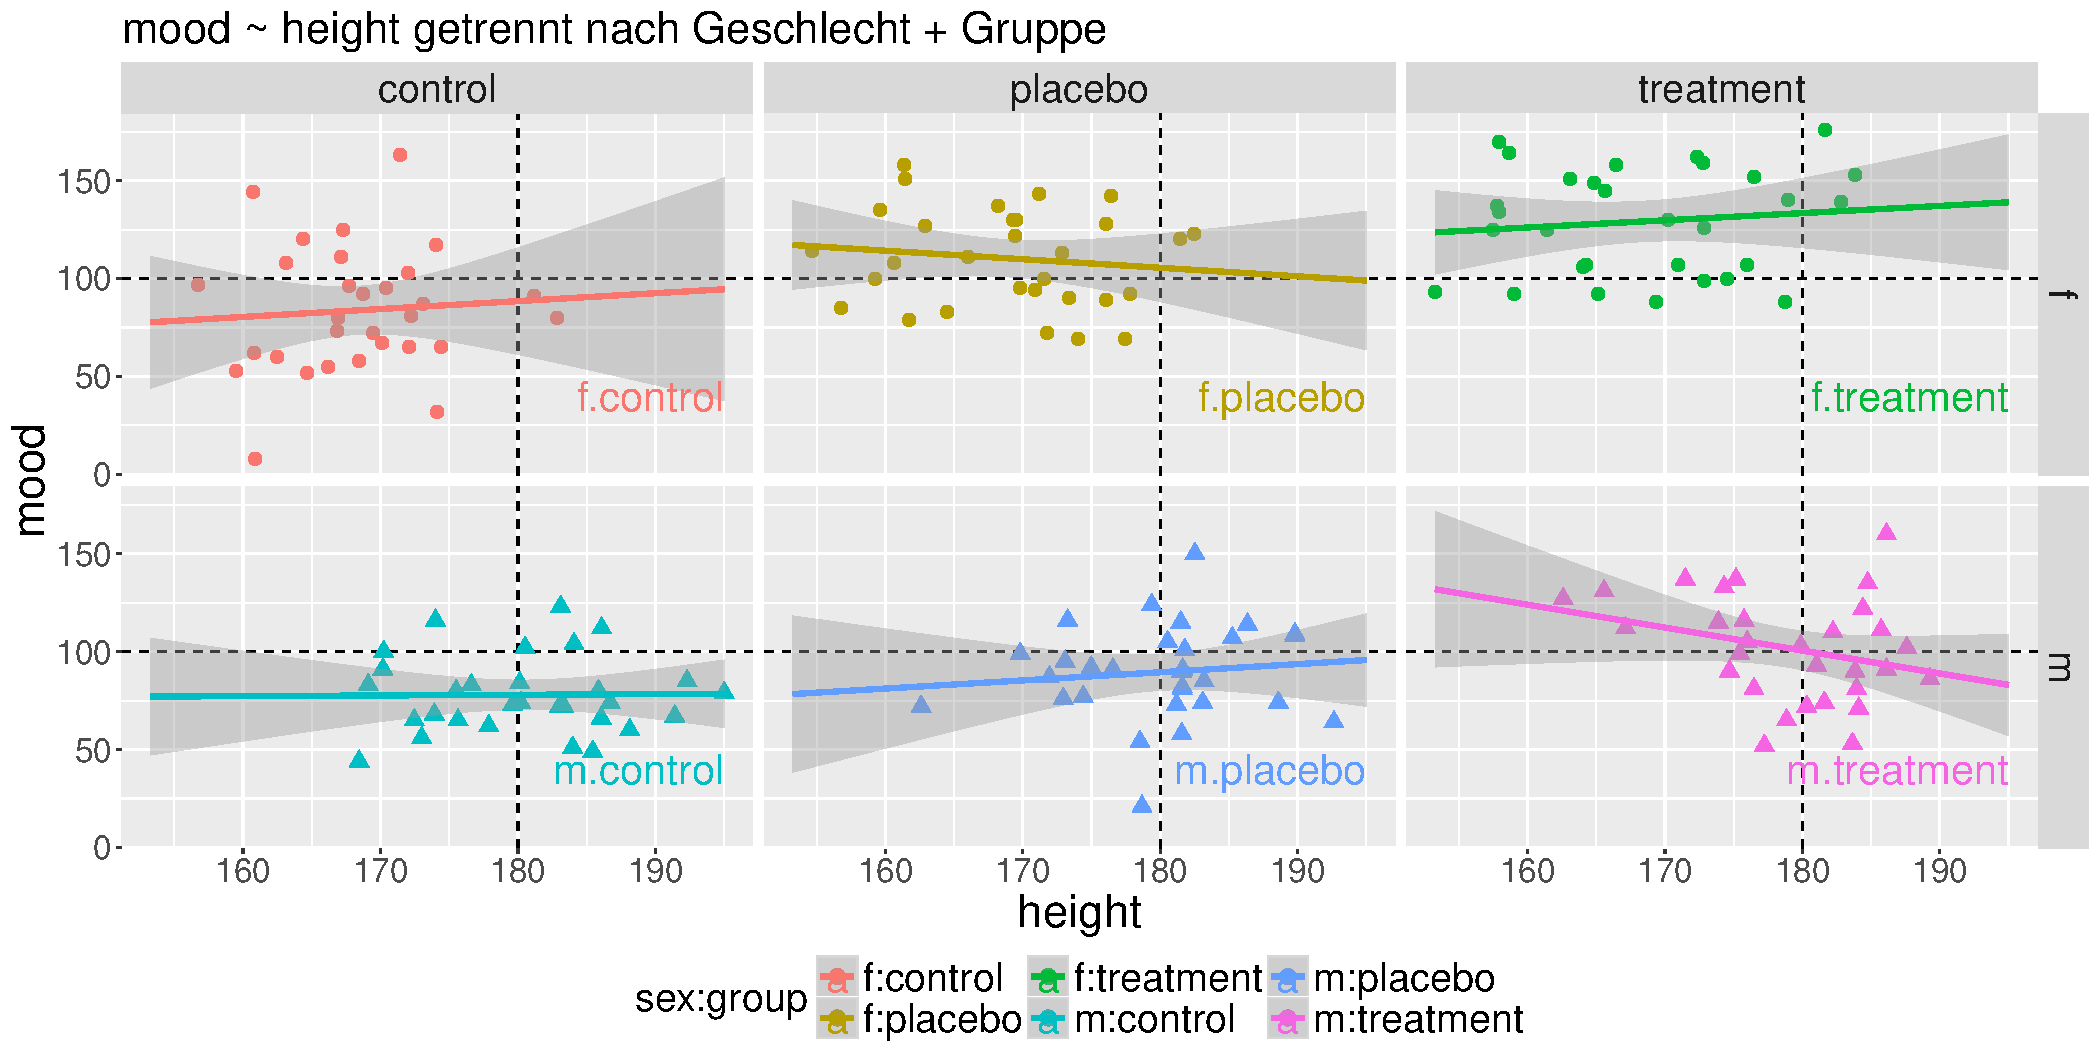
\includegraphics[width=12.5cm]{ggplot09}
\vspace*{-0.5em}
\caption{Angepasste Position und Einträge der Legende mit \lstinline!guides()! sowie \lstinline!theme()!}
\label{fig:ggplot09}
\end{figure}

%%%%%%%%%%%%%%%%%%%%%%%%%%%%%%%%%%%%%%%%%%%%%%%%%%%%%%%%%%%%%%%%%%
%%%%%%%%%%%%%%%%%%%%%%%%%%%%%%%%%%%%%%%%%%%%%%%%%%%%%%%%%%%%%%%%%%
\subsection{Farben, Datenpunktsymbole und Linientypen}
\label{sec:ggplotColour}
%%%%%%%%%%%%%%%%%%%%%%%%%%%%%%%%%%%%%%%%%%%%%%%%%%%%%%%%%%%%%%%%%%
%%%%%%%%%%%%%%%%%%%%%%%%%%%%%%%%%%%%%%%%%%%%%%%%%%%%%%%%%%%%%%%%%%

Farben, Datenpunktsymbole und Linientypen lassen sich auf zwei Wegen wählen: Entweder werden diese visuellen Attribute im Aufruf von \lstinline!ggplot()! bzw.\ von \lstinline!geom_<<Name>>()! innerhalb von \lstinline!aes()! mit Variablen eines Datensatzes verknüpft, oder aber außerhalb von \lstinline!aes()! auf einen festen Wert gesetzt.
\begin{itemize}
\item Für Farben existiert das Argument \lstinline!colour! (für mögliche Werte s.\ Abschn.\ \ref{sec:colors}). Zusätzlich zu \lstinline!colour! kann \lstinline!alpha! mit Zahlen im Bereich von 0--1 den Grad der simulierten Transparenz festlegen. Dies kann etwa sinnvoll sein, wenn Diagrammelemente übereinander plaziert werden sollen, ohne dass später gezeichnete Elemente früher gezeichnete vollständig verdecken.
\item Die Datenpunktsymbole eines Punktdiagramms bestimmt \lstinline!shape! (für mögliche Werte s.\ Abschn.\ \ref{sec:par}).
\item Für Linientypen eines Liniendiagramms ist \lstinline!linetype! vorgesehen (mögliche Werte sind \lstinline!"solid"!, \lstinline!"dashed"!, \lstinline!"dotted"! oder die in Abschn.\ \ref{sec:par} genannten Zahlen).
\item Die Größe der Datenpunkte gibt \lstinline!size! vor, die Dicke der Punktumrisse \lstinline!stroke! und die Linienbreite ebenfalls \lstinline!size!. 
\end{itemize}

Bei der Zuordnung von Farben zu Variablen existiert eine große Vielfalt von Gestaltungsmöglichkeiten, die sich aus dem möglichen Austausch der verwendeten Farbpaletten ergibt. Dazu fügt man der Grundschicht eine der folgenden Schichten mit \lstinline!+! hinzu:
\begin{itemize}
\item \index[func]{scale_colour_hue()@\lstinline{scale_colour_hue()}} \lstinline!scale_colour_hue(h=<<Farbton>>, c=<<Sättigung>>, l=<<Helligkeit>>)! ist die Voreinstellung und sorgt für annähernd gleich helle Farben unterschiedlichen Farbtons. Die Farben lassen sich bzgl.\ des abgedeckten Farbbereichs (Vektor \lstinline!h! von zwei Winkeln im Farbkreis 0--360), der vom Farbton abhängigen Sättigung \lstinline!c! und der Helligkeit \lstinline!l! (0--100) modifizieren. Andere Farbgradienten erzeugt \index[func]{scale_colour_gradient()@\lstinline{scale_colour_gradient()}} \lstinline!scale_colour_gradient()!.
\item \index[func]{scale_colour_grey()@\lstinline{scale_colour_grey()}} \lstinline!scale_colour_grey(start=0.2, end=0.8)! stellt Linien und Umrisse in Graustufen im Bereich von \lstinline!start! bis \lstinline!end! dar, wobei der mögliche Wertebereich jeweils von 0--1 reicht.
\item Das im Basisumfang von R enthaltene Paket \index[pack]{colorspace@\lstinline{colorspace}} \lstinline!colorspace! verfügt über eine Reihe von Farbpaletten, die für unterschiedliche Zwecke optimiert sind -- etwa zur Visualisierung stetiger Übergänge, zur besseren Unterscheidbarkeit unterschiedlicher Gruppen oder für Ausdrucke in Graufstufen. Zu diesen Paletten wechseln Funktionen, deren Namen analog zu \index[func]{scale_color_continuous_sequential()@\lstinline{scale_color_continuous_sequential()}} \lstinline!scale_color_continuous_sequential()! oder \index[func]{scale_fill_discrete_qualitative()@\lstinline{scale_fill_discrete_qualitative()}} \lstinline!scale_fill_discrete_qualitative()! aufgebaut sind. Das Argument \lstinline!palette! erlaubt es dabei, zwischen mehreren Varianten zu wählen.\footnote{\url{http://colorspace.r-forge.r-project.org/articles/ggplot2_color_scales.html} zeigt Details und Beispiele.} Alle Funktionen nach dem Muster \lstinline!scale_color_<<...>>()! legen Farben für Linien und Umrisse fest. Die Farbe gefüllter Flächen wird analog über die zugehörigen Funktionen \lstinline!scale_fill_<<...>>()! definiert.
\end{itemize}

Nun soll die Größe der Datenpunktsymbole sowie der Linientyp angepasst werden (Abb.\ \ref{fig:ggplot10}).
\begin{lstlisting}
> ggplot(groupM, aes(x=group, y=mood, color=sex, shape=sex, group=sex)) +
+     geom_point(size=8, stroke=2) +
+     geom_line(size=2, linetype="dashed") +
+     scale_shape_discrete(solid=FALSE)
\end{lstlisting}

Das folgende nach Gruppen getrennte Histogramm mit Kerndichteschätzer verwendet eine der \lstinline!colorspace! Farbpaletten und setzt simulierte Transparenz für eine bessere Sichtbarkeit der einzelnen Flächen in sich überlappenden Regionen ein (Abb.\ \ref{fig:ggplot10}).
\begin{lstlisting}
> library(colorspace)           # für scale_fill_discrete_qualitative()
> ggplot(myDf, aes(x=mood, fill=group)) +
+     geom_histogram(aes(y=..density..), alpha=0.5) +
+     geom_density(alpha=0.7) +
+     scale_fill_discrete_qualitative()
\end{lstlisting}

\begin{figure}[ht]
\centering
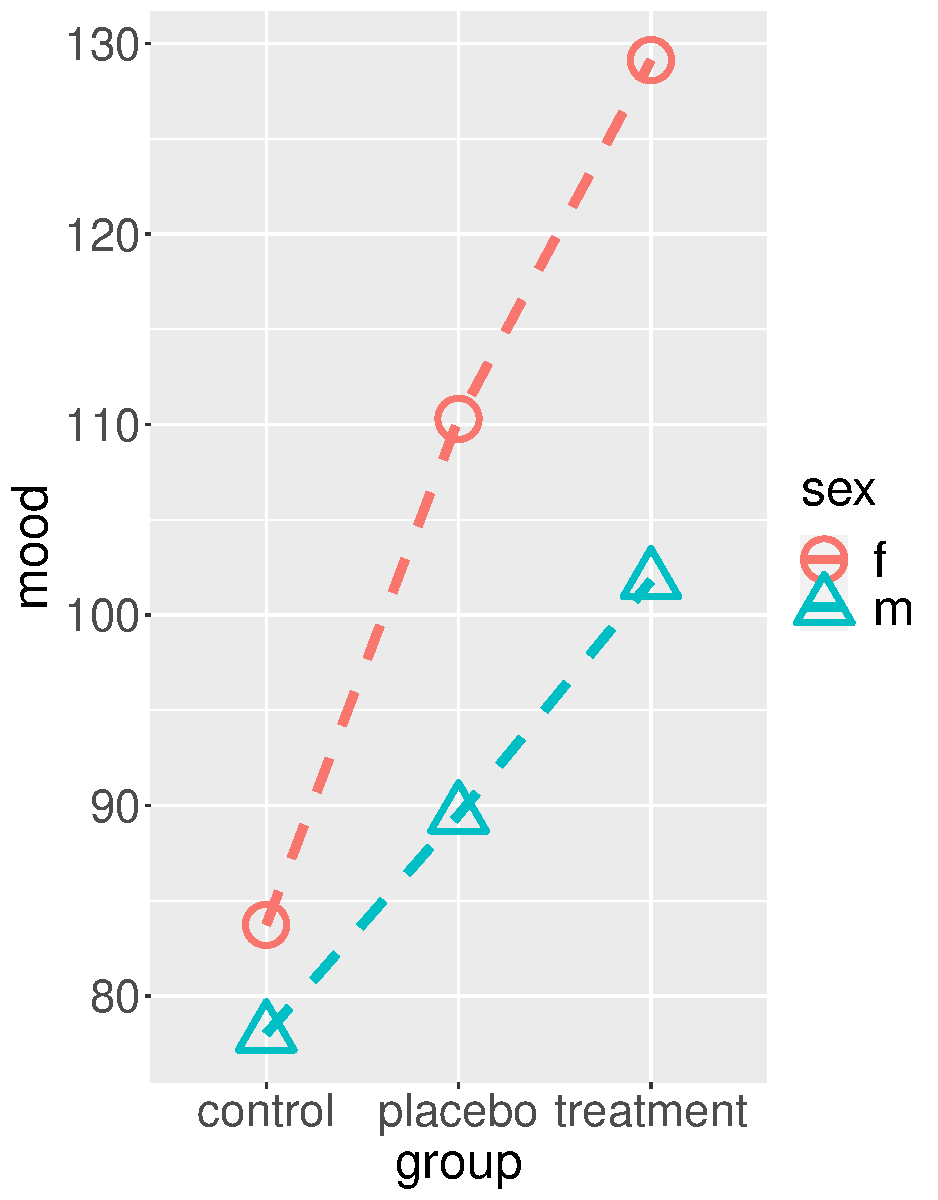
\includegraphics[width=6.25cm]{ggplot10a}
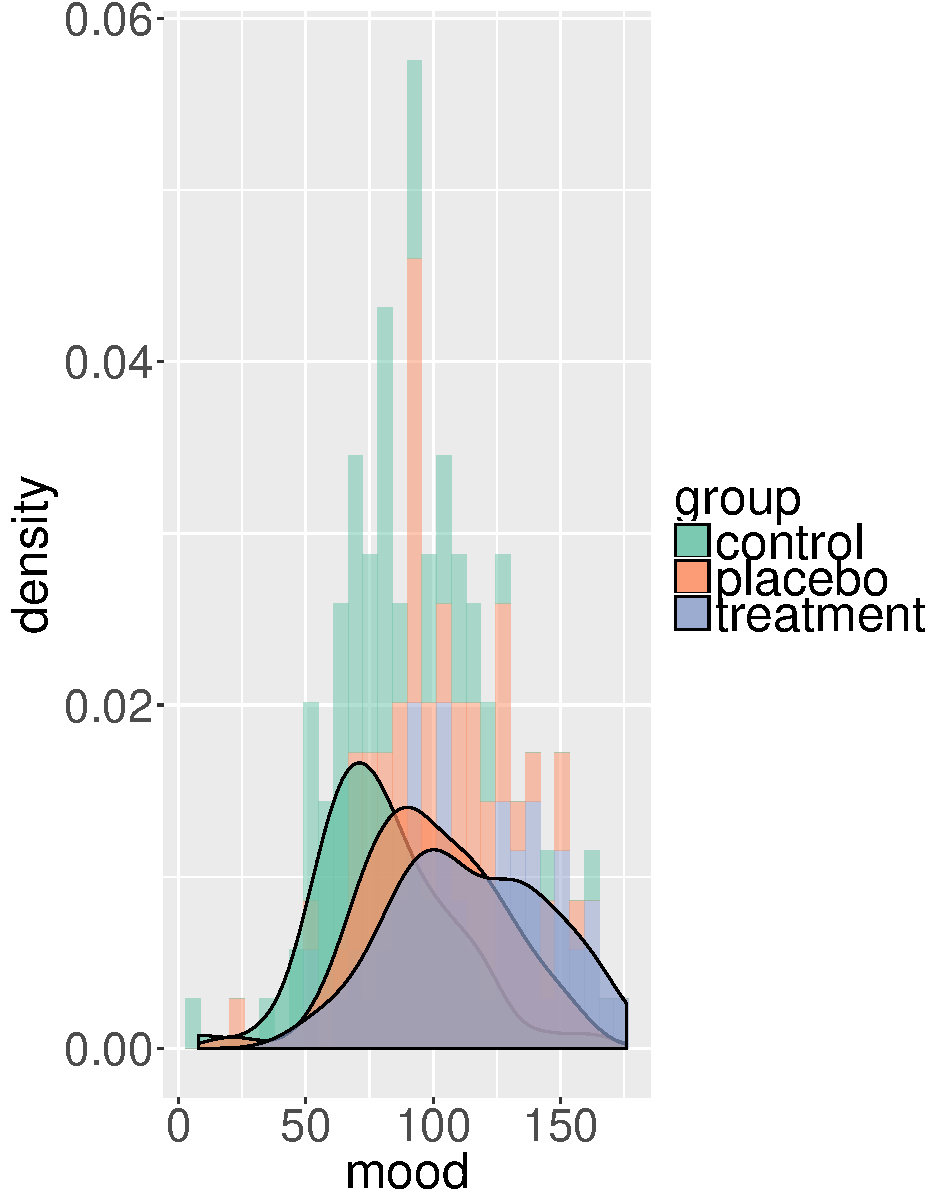
\includegraphics[width=6.25cm]{ggplot10b}
\vspace*{-0.5em}
\caption{Angepasste Datenpunktsymbole, Linientypen und Farben mit \lstinline!scale_shape_discrete()! und \lstinline!scale_fill_discrete_qualitative()!}
\label{fig:ggplot10}
\end{figure}

%%%%%%%%%%%%%%%%%%%%%%%%%%%%%%%%%%%%%%%%%%%%%%%%%%%%%%%%%%%%%%%%%%
%%%%%%%%%%%%%%%%%%%%%%%%%%%%%%%%%%%%%%%%%%%%%%%%%%%%%%%%%%%%%%%%%%
\subsection{Aussehen im Detail verändern}
\label{sec:ggplotTheme}
%%%%%%%%%%%%%%%%%%%%%%%%%%%%%%%%%%%%%%%%%%%%%%%%%%%%%%%%%%%%%%%%%%
%%%%%%%%%%%%%%%%%%%%%%%%%%%%%%%%%%%%%%%%%%%%%%%%%%%%%%%%%%%%%%%%%%

Um Details im Aussehen von \lstinline!ggplot2!-Diagrammen zu ändern, kann man auf zwei Wegen vorgehen: Eine mit \lstinline!+! zu einer Grundschicht hinzugefügte \lstinline!theme_<<Name>>()! Schicht verändert gleichzeitig viele Einstellungen, die den grundsätzlichen Diagrammstil bestimmen:\footnote{Weitere stellt das Paket \index[pack]{ggthemes@\lstinline{ggthemes}} \lstinline!ggthemes! \cite{Arnold2016} zur Verfügung.}
\begin{itemize}
\item \index[func]{theme()@\lstinline{theme()}}\lstinline!theme_grey()! ist die Voreinstellung und sorgt für einen leicht grauen Hintergrund der ohne Rahmen dargestellten Zeichnungsfläche, auf der dünne weiße Gitterlinien zu sehen sind.
\item \index[func]{theme_bw()@\lstinline{theme_bw()}}\lstinline!theme_bw()! setzt den Hintergrund der Zeichnungsfläche auf weiß und rahmt sie mit einer dünnen schwarzen Linie ein. Die Gitterlinien sind grau.
\item \index[func]{theme_minimal()@\lstinline{theme_minimal()}}\lstinline!theme_minimal()! entfernt gegenüber \lstinline!theme_bw()! den Rahmen um die Zeichnungsfläche und um Elemente der Legende. Linien für die Achsen fehlen ebenfalls.
\item \index[func]{theme_classic()@\lstinline{theme_classic()}}\lstinline!theme_classic()! entfernt gegenüber \lstinline!theme_minimal()! noch alle Gitterlinien.
\end{itemize}

Eine Reihe von optischen Details wie Schriftgröße, -art und -farbe des Titels, der Achsenbeschriftungen und der Legende lassen sich zudem auch einzeln mit \index[func]{theme()@\lstinline{theme()}}\lstinline!theme()! verändern. Diese Funktion kontrolliert u.\,a.\ auch die Randgrößen sowie die Farbe der Panel-Beschriftungen und Gitterlinien. Alle Einstellmöglichkeiten erläutert \lstinline!?theme!.

Die in Abb.\ \ref{fig:ggplot11} gezeigten Diagramme reduzieren die visuellen Elemente von Abb.\ \ref{fig:ggplot10} aus Abschn.\ \ref{sec:ggplotColour} sowie von Abb.\ \ref{fig:ggplot08bc} aus Abschn.\ \ref{sec:ggplotAxis}.
\begin{lstlisting}
> library(colorspace)           # für scale_fill_discrete_qualitative()
> ggplot(myDf, aes(x=mood, fill=group)) +
+     geom_histogram(aes(y=..density..), alpha=0.5) +
+     geom_density(alpha=0.7) +
+     scale_fill_discrete_qualitative() +
+     theme_bw())

> ggplot(myDf, aes(x=sex, y=height, fill=sex)) +
+     geom_boxplot() +
+     coord_flip(ylim=c(140, 200)) +
+     theme_minimal()
\end{lstlisting}

\begin{figure}[ht]
\centering
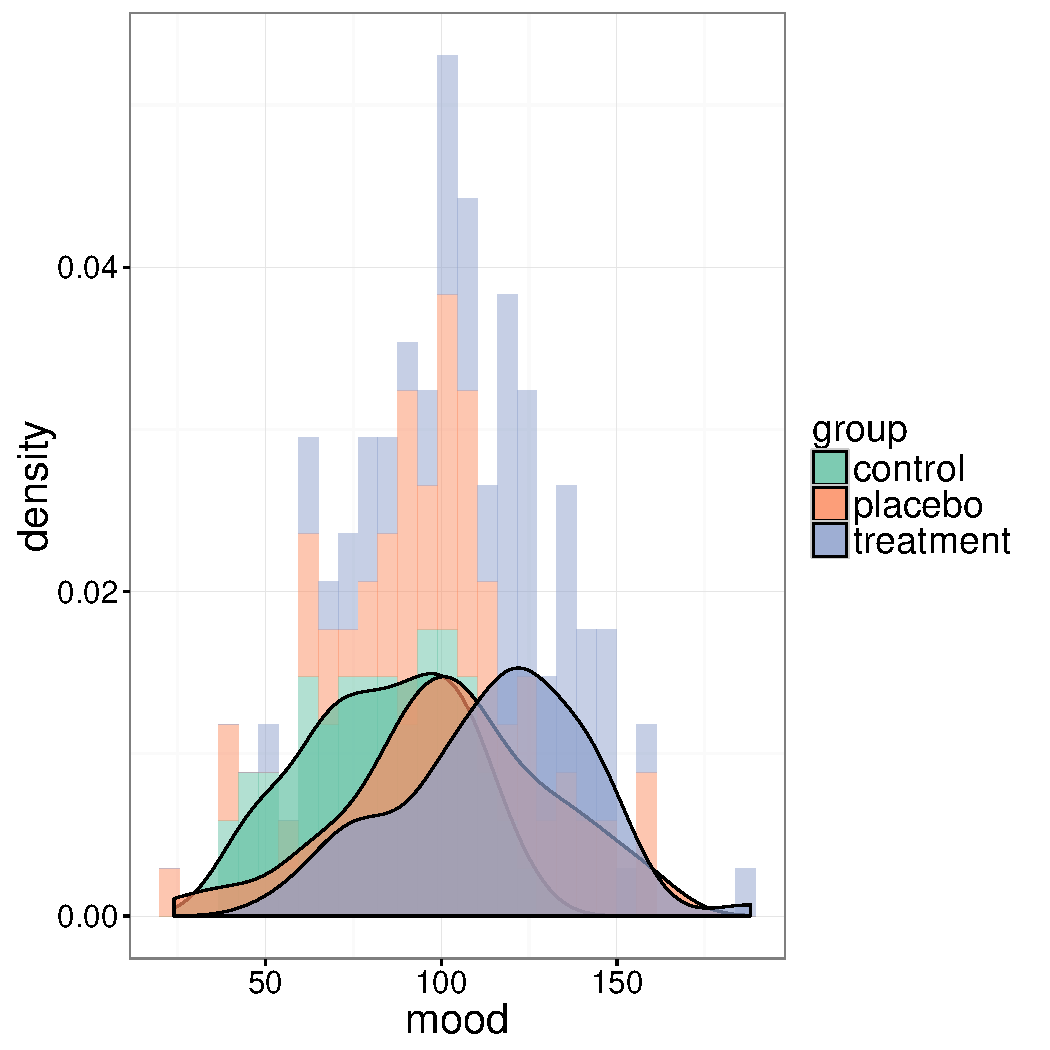
\includegraphics[width=6.25cm]{ggplot11a}
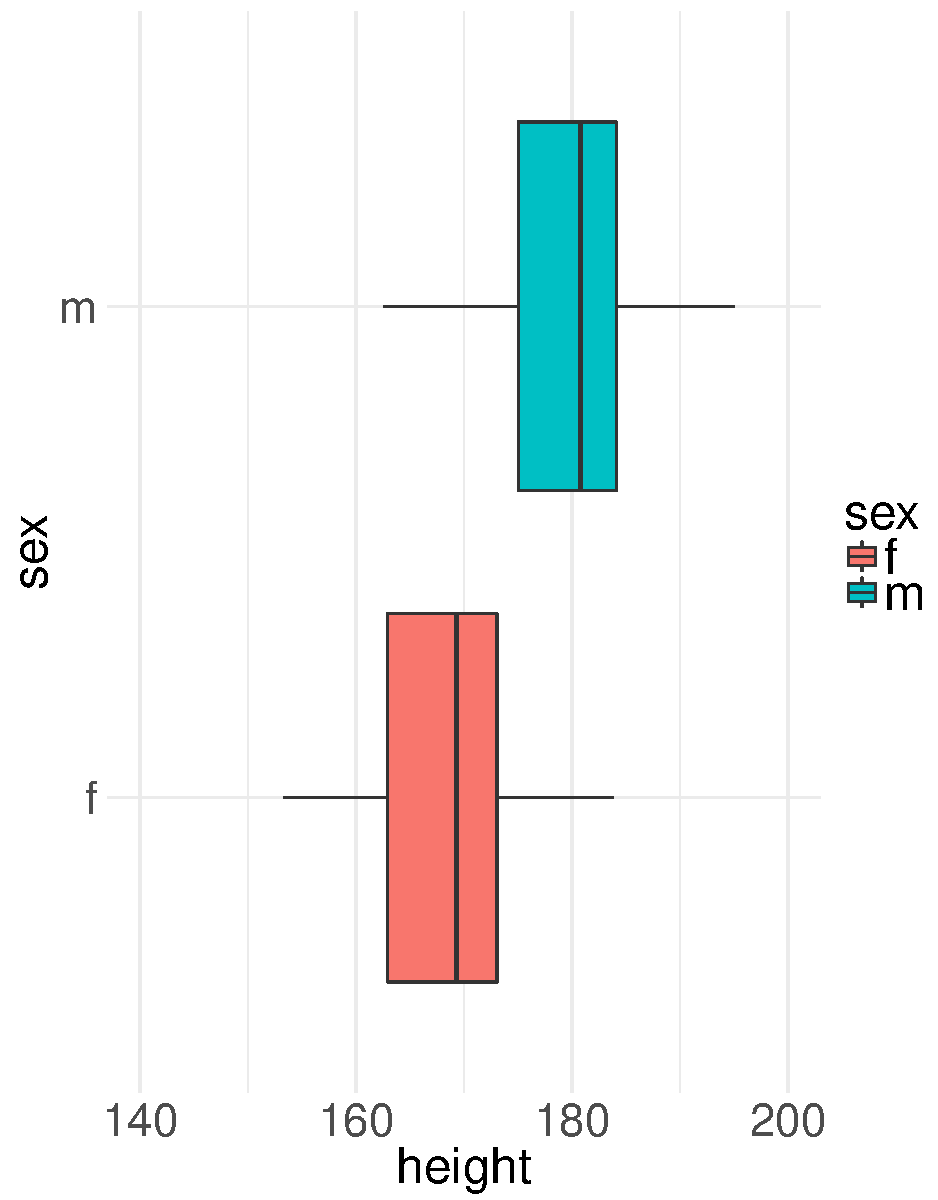
\includegraphics[width=6.25cm]{ggplot11b}
\vspace*{-0.5em}
\caption{Reduzierte Diagrammelemente mit \lstinline!theme_bw()! sowie \lstinline!theme_minimal()!}
\label{fig:ggplot11}
\end{figure}
